\documentclass[12pt]{article}
\usepackage[utf8]{inputenc}
\usepackage{graphicx}
\graphicspath{ {images/} }
\usepackage[sorting=none]{biblatex}
\usepackage{amsmath}
\usepackage{titlesec}
\usepackage{subcaption}
\addbibresource{references.bib}
\usepackage{geometry}
 \geometry{
 a4paper,
 total={170mm,257mm},
 left=20mm,
 top=20mm,
 }

\begin{document}

\begin{titlepage}
   \begin{center}
       \vspace*{1cm}

       \textbf{The Formal Grammar of Foliage:  L-Systems for Procedural Generation of Computer Graphics}

       \vspace{0.5cm}
IS71021E Assignment 1 

            
       \vspace{1.5cm}

       \textbf{Oliver J. Martin}
\\MSc Computer Games Programming
       \vfill
            
       
    
       
\includegraphics[width=0.4\textwidth]{Tree}

\vfill
            
\vspace{0.7cm}

       Department of Computing\\
       Goldsmiths, University of London\\
\today
            
   \end{center}
\end{titlepage}

\section{Introduction}
Despite originating as a mathematical theory for the development of filamentous organisms \cite{lindenmayer}, the introduction of Lindenmayer systems (or L-systems) inspired a range of geometric interpretations with the aim of procedurally modelling complex branching structures such as plants and fractals \cite{graphical}. In the ensuing decades, L-systems have been used in the modelling an ever-expanding range of structures - from city maps \cite{city} to virtual creatures \cite{hornby}. \\
This paper describes an implementation of an L-system using Unity and the C\# programming language. This system is capable of generating models in both 2D and 3D, as well as the incorporation of a lineage-based parametric system as first described in \cite{Hanan}. 

\section{Methods}
\subsection{Parallel Rewriting}
L-Systems are a type of string-rewriting mechanism, whereby a complex string is derived by successively replacing components of a simple initial string - with a set of production rules defining the replacements.  As opposed to the sequential application of rules in Chomsky's earlier work on string rewriting \cite{chomsky},  L-systems utilise \textit{parallel rewriting} - where production rules are applied simultaneously to the entirety of the input string \cite{lindenmayer}, opening up the possibility of generating more complex structures.\\
\subsection{Turtle Geometry}
To generate an image from the string generated by the L-system, a relative cursor known as a \textit{turtle} is used to interpret each character of the final string in order - with different symbols representing different commands \cite{graphical}. In the simplest case, the state of the turtle at each point is represented as a triplet \((x, y, z, \alpha)\) where \((x, y, z)\) is the current position of the turtle and \(\alpha\) represents the orientation of the turtle. 

\subsubsection{Orientation}
In 2D, the orientation \(\alpha\) can be represented by a single angle. However, to expand the capability of the system to generate 3D structures, the representation of the turtle's current orientation must be expanded to 3 orthonormal vectors \(\vec{H}\),\(\vec{L}\) and \(\vec{U}\) - representing the heading of the turtle, the direction to the left, and the direction up respectively \cite{turtle}. 

\subsubsection{Rotation and Moving}
Rotations of angle \(\delta\) around each axis of the turtle's orientation are given by the following rotation matrices:
\begin{equation*}
R_{\vec{H}}(\delta) = \begin{bmatrix}cos\,\delta&sin\,\delta&0\\-sin\,\delta&cos\,\delta&0\\0&0&1 \end{bmatrix}
\end{equation*}
\begin{equation*}
R_{\vec{L}}(\delta) = \begin{bmatrix}cos\,\delta&0&-sin\,\delta\\0&1&0\\sin\,\delta&0&cos\,\delta \end{bmatrix}
\end{equation*}
\begin{equation*}
R_{\vec{U}}(\delta) = \begin{bmatrix}1&0&0\\0&cos\,\delta&-sin\,\delta\\0&sin\,\delta&cos\,\delta \end{bmatrix}
\end{equation*}
Representing the orientation axes as row vectors, the new orientation following a rotation can then be expressed as:
\begin{equation}
\begin{bmatrix} \vec{H}' \\ \vec{L}' \\ \vec{U}' \end{bmatrix}=R
\begin{bmatrix}
	H_{x} & H_{y} & H_{z}\\
	L_{x} & L_{y} & L_{z}\\
	U_{x} & U_{y} & U_{z}\\
\end{bmatrix}
\end{equation}
The new position of the turtle, \((x', y', z')\) following a move forward of step size \textit{d} can then be calculated as:
\begin{equation}
	(x', y', z') = (x, y, z) + d\vec{H}
\end{equation}

The following operations are then used to control the turtle:

\begin{center}
\begin{tabular}{c p{8cm}}
DRAW& Move forward and draw a line \\\\
TURN& Rotate about \(\vec{U}\), using \(R_{\vec{U}}\). The only rotation used in 2D systems.\\\\
PITCH&Rotate about \(\vec{L}\), using \(R_{\vec{L}}\). \\\\
ROLL&Rotate about \(\vec{H}\), using \(R_{\vec{H}}\). \\\\
HORIZONTAL&Rotate turtle about its axis such that \(\vec{U}\) is \((0,1,0)\).
\end{tabular}
\end{center}

\subsubsection{Bracketed Systems}
To achieve branching structures, a \textit{bracketed} L-system is implemented. A \textit{stack} is created and two new stack operations are introduced:\\

\begin{center}
\begin{tabular}{l p{8cm}}
PUSH& Push the current turtle state onto the stack.\\\\
POP& Pop the top state from the stack and make it the current state of the turtle.
\end{tabular}
\end{center}
Typically, the push operation is represented with an opening square bracket ( [ ) and the pop operation with a closing square bracket ( ] ) - which together bracket and delimit branches within the string.
\subsection{Edge and Node Rewriting}
When using an L-system with turtle graphics, there are two common modes of operation - node and edge rewriting.  Edge rewriting is simply replacing each edge (i.e. each symbol which represents a draw command) with a new sequence, while node rewriting involves replacing characters that are not graphically or physically relevant to the system (i.e. are ignored by the turtle) - with these characters instead being considered logically relevant and representing subfigures.
\subsection{Parametric L-Systems}
Parametric L-systems extend the capabilities of L-systems by associating numerical parameters with letters, which can control physical constants such as line length, line width, or rotation angle \cite{Hanan}. This allows for continuous processes (such as a plant growing) to be modelled, as information can flow through the system as it ``grows". 
\subsection{Implementation}
The L-system was created primarily in C\#, with the Unity game engine used to draw lines, create UI, and handle user inputs.
\subsubsection{Objectives}
\begin{itemize}
\item Read a configuration file containing L-system parameters, and display the result.
\item Allow user input to control selected L-system, current iteration, and L-system parameters.
\item Allow full customisation of symbols and commands within the configuration file.
\item Extend L-system functionality into 3D.
\item Implement parametric L-system functionality.
\end{itemize}
\subsubsection{Classes}

\paragraph{{\large\texttt{LSystem}}}\mbox{} \\
Loads configuration files, runs the text replacement algorithm, and handles user input. For each loaded config file, the \texttt{RunSystem} function is run. For each iteration, this function instantiates a \texttt{Turtle} object, calls the \texttt{RunIteration} function, and gets that iteration's \texttt{Turtle} to draw the resulting string.\\
The \texttt{RunIteration} function takes the an initial string and a dictionary containing the production rules as inputs and computes the result of applying the rules. To do this, an empty ``output" string is initialised and each character in the string is looped through. Each character is checked against the keys of the rules dictionary - if it exists as a key the associated value is appended to the output string (i.e. replacing that character with its rules), otherwise the original character is appended.\\
To propagate the parameters through the iterations, each character through the string actually checks the preceding character against the rules. In the case that an open bracket is the current character, the preceding character is stored until a closing bracket is encountered - with the current ``parameter" values in between being added to a separate empty string in the meantime. Once the closing bracket is found, the relevant parameter values are found within the rule for the preceding character by performing a Regex match for any characters found between brackets. These values are then replaced with a custom match evaluator that splits the attributes by comma,  multiplies the current attribute and the value in the rule together, and then reforms the correct format with the values separated by commas. This updated rule is then added to the output string, which ensures the updated parameters are passed to the next iteration.\\
Once this process has been completed for the entire original string, the output string is returned. 
\pagebreak
\paragraph{{\large\texttt{Turtle}}}\mbox{} \\
Handles the drawing of one iteration of a given L-system, given its string. Each turtle takes one string and a dictionary containing the commands associated with different characters as inputs, and starts by instantiating an initial \texttt{Line} object. Sequentially, each character in the string is checked against the commands dictionary. If a command is found, a switch statement checks the command's \texttt{type} property against the \texttt{CommandType.TYPES} enum to determine what type of operation to perform. \\ Similarly to the \texttt{RunIteration} function, drawing is paused if an open bracket is encountered until the next closed bracket. Again, this reads the parameters found between the brackets and either multiplies the \texttt{amount} property of the command by the parameter (in the case of a length or angle parameter), or changes the width of the line at the current point (in the case of a width parameter).\\ For each character, the current position is stored as a \texttt{TurtlePoint} data structure - which can be added and retrieved from a stack of \texttt{TurtlePoints} if bracket commands are encountered. When a pop command is encountered, a new \texttt{Line} object is created as the new active line and is initialised with the popped \texttt{TurtlePoint} state. \\
The \texttt{HandleForward} method calculates the updated position of the turtle by utilising equation 2, and also updates the width of the line if it has been changed by a parameter - both of which are passed to the currently active \texttt{Line}. \\ The \texttt{HandleRotation} method constructs the correct rotation matrix from section 2.2.2, depending on the \texttt{type} property of the current command, this is then passed to the \texttt{Rotate} function of the current \texttt{TurtleOrientation} to calculate the new orientation of the turtle.  The \texttt{HandleHorizontal} function rotates the turtle about its axis so that t \(\vec{U}\) is \((0,1,0)\). To do this it uses the following equations:
\begin{equation*}
\vec{L} = \frac{\vec{V} \times \vec{H}}{|\vec{V} \times \vec{H}|}
\end{equation*}
\begin{equation*}
\vec{U} = \vec{H} \times \vec{L}
\end{equation*}
where \( \vec{V}\) is the global up direction.

\paragraph{{\large\texttt{Line}}}\mbox{} \\
The \texttt{Line} class primarily functions as an instantiable wrapper for the \texttt{LineRenderer} built-in class. It also handles processing the line width. When a point is added with a custom width, it is added to a \texttt{widths} dictionary - with its key being the cumulative length to that point along the line. When the line is completed, the \texttt{widthCurve} attribute of the \texttt{LineRenderer} is calculated - with the \(x\) value of each point being the proportional length of each point (i.e. the total length to that point divided by the length of the whole line), and the \(y\) value being the desired width. This ensures that each branch reduces in width at the correct rate.
\pagebreak
\subsubsection{Data Structures}

\paragraph{{\large\texttt{Config}}}\mbox{} \\
Contains the configuration details of an L-system.\\\\
\textbf{Properties: }
\begin{center}
\begin{tabular}{c p{12cm}}
\texttt{name}& A string representing the name of the L-system.\\
\texttt{variables}& A list of strings containing the variables of the L-system.\\
\texttt{constants}& A list of strings containing the constants of the L-system. \\
\texttt{axiom}& A string representing the initial state of the L-system. \\
\texttt{rules}& A list of \texttt{ProductionRule} data structures containing the rules of the system. \\
\texttt{commands} & A list of \texttt{Command} data structures containing the operations associated with each symbol.\\
\texttt{n} & The integer number of iterations to compute.\\
\texttt{lineWidth} & The base line width, stored as a float.\\
\end{tabular}
\end{center}
\textit{Note: Symbols are represented as strings rather than characters for use in parametric systems, as well as potential future implementation of context-sensitivity. Additionally, Unity is not capable of serialising dictionaries, so both the \texttt{rules} and \texttt{commands} field act as wrappers which are later unwrapped into dictionaries for reduced time complexity.}\\

The configuration is typically defined by a JSON configuration file. JSON was chosen as the format primarily due to its human-readability, as advanced system customisation through modifying configuration files was one of the objectives. The JSON file must contain all the fields detailed above.
\paragraph{{\large\texttt{ProductionRule}}}\mbox{} \\
Contains a production rule for a given L-system.\\\\
\textbf{Properties: }
\begin{center}
\begin{tabular}{c p{12cm}}
\texttt{key}& A string representing the character(s) to be replaced for a rule. If this is intended to be used as a module in a parametric system, the symbol should be followed by ``()" (e.g. F()).\\
\texttt{value}& The value to replace the key with.\\
\end{tabular}
\end{center}

\paragraph{{\large\texttt{Command}}}\mbox{} \\
Contains a single command for a given L-system.\\\\
\textbf{Properties: }
\begin{center}
\begin{tabular}{c p{12cm}}
\texttt{key}& A string representing the indicator for the turtle to perform this command.\\
\texttt{type}& A \texttt{CommandType} value defining the type and amount of this command.\\
\end{tabular}
\end{center}
\pagebreak
\paragraph{{\large\texttt{CommandType}}}\mbox{} \\
Represents the type of a given command, and how much of that command to perform.\\\\
\textbf{Properties: }
\begin{center}
\begin{tabular}{c p{12cm}}
\texttt{type}& A value from the \texttt{TYPES} enum to define the type of the command.\\
\texttt{amount}& A float defining the base amount of this command to perform (i.e. step size for a move command, angle for a rotation).\\
\end{tabular}
\end{center}
This class also contains the \texttt{TYPES} enum, which enumerates the different types of commands:\\
\begin{center}
\begin{tabular}{c c}
0&\texttt{DRAW}\\
1&\texttt{TURN}\\
2&\texttt{POP}\\
3&\texttt{PUSH}\\
4&\texttt{PITCH}\\
5&\texttt{ROLL}\\
6&\texttt{HORIZONTAL}\\
\end{tabular}
\end{center}


\paragraph{{\large\texttt{TurtlePoint}}}\mbox{} \\
Represents the state of a turtle.\\\\
\textbf{Properties: }
\begin{center}
\begin{tabular}{c p{12cm}}
\texttt{position}& The current position of the turtle represented as a Vector3.\\
\texttt{orientation}& A \texttt{TurtleOrientation} representing the current orientation.\\
\texttt{lineWidth}& The width of the line as a float.\\
\end{tabular}
\end{center}
\paragraph{{\large\texttt{TurtleOrientation}}}\mbox{} \\
Contains the vectors \(\vec{H}\), \(\vec{L}\), and \(\vec{U}\) for a turtle. Handles the calculation for rotations.\\\\
\textbf{Properties: }
\begin{center}
\begin{tabular}{c p{12cm}}
\texttt{heading}& \(\vec{H}\) represented as a Vector3.\\
\texttt{left}& \(\vec{L}\) represented as a Vector3.\\
\texttt{up}& \(\vec{U}\) represented as a Vector3.\\
\end{tabular}
\end{center}\mbox{} \\\\
\textbf{Methods: }
\begin{center}
\begin{tabular}{c p{12cm}}
\texttt{Rotate}&Takes a 3x3 rotation matrix as an input, multiplies the rotation matrix by the current coordinate frame and returns the result as a a new \texttt{TurtleOrientation}\\
\end{tabular}
\end{center}


\subsubsection{User Controls}
\paragraph{Hot Keys}\mbox{}
\begin{center}
\begin{tabular}{c c}
Right Arrow/D& Increment Iteration\\
Left Arrow/A& Decrement Iteration\\
Up Arrow/W& Next L-system\\
Down Arrow/S& Previous L-system\\
Scroll Wheel Up& Zoom Camera In\\
Scroll Wheel Down&Zoom Camera Out
\end{tabular}
\end{center}
\paragraph{GUI}\mbox{}\\\\
Within the GUI, the user can modify any of the operations for the currently viewed L-system. This is done by selecting the desired parameter to change with the drop-down menu and then changing the value in the input field below. The system automatically redraws when the change is confirmed.

\section{Results}
For these results, the following symbols are used as commands:

\begin{center}
\begin{tabular}{c c}
F& Move Forwards and Draw\\\relax
[& Push Current State to Stack\\\relax
]& Pop State From Stack\\
+& Turn (Positive)\\
-& Turn (Negative)\\\relax
\&& Pitch (Positive) \\\relax
\^& Pitch(Negative)\\\relax
\textbackslash& Roll (Positive)\\
/& Roll (Negative)\\
|& Turn $180^{\circ}$ \\
\$&  Set Up Vector to (0,1,0)
\end{tabular}
\end{center}

\subsection{2D Plant-Like Structures}
Figure 1 shows three plant-like structures generated by edge-rewriting L-systems, while figure 2 shows three-plant like structures generated by node-rewriting systems. Both figures use bracketed systems, which creates the branching structure that they demonstrate. 

\begin{figure}
\begin{subfigure}{1\textwidth}
\centering
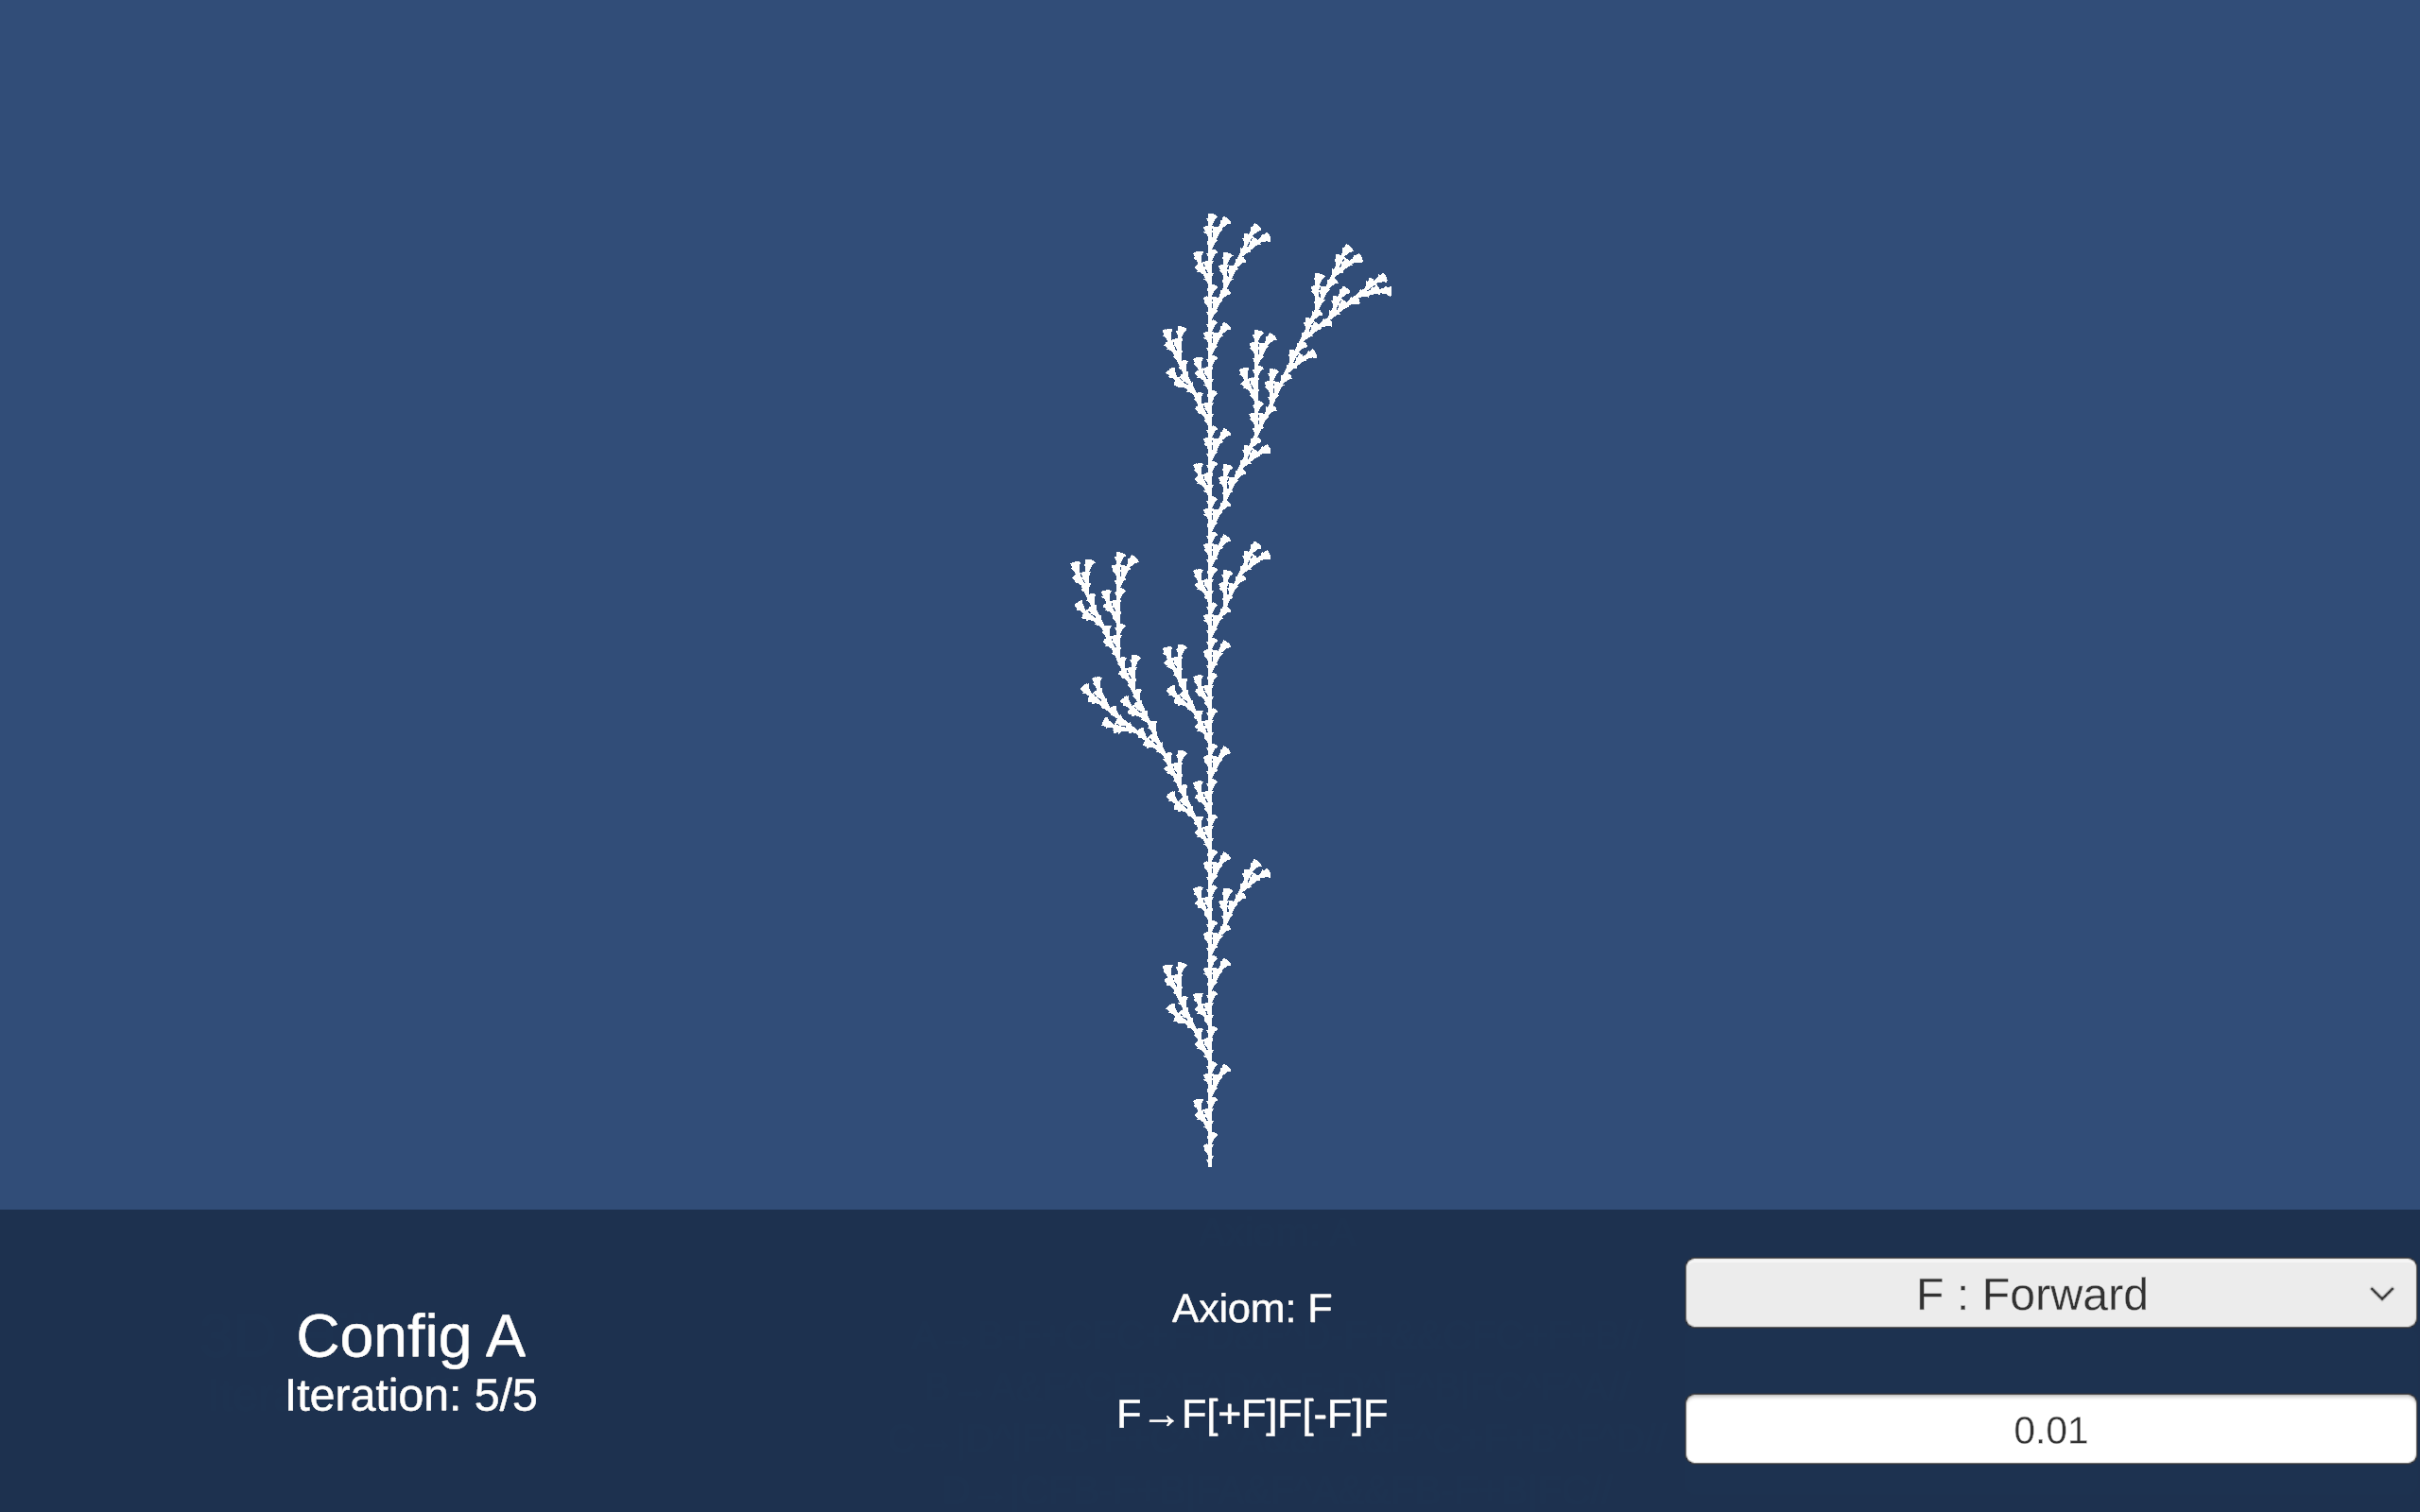
\includegraphics[width=.7\linewidth]{A.png}
\caption{$\delta$ = 25.7$^{\circ}$}
\end{subfigure}
\begin{subfigure}{1\textwidth}
\centering
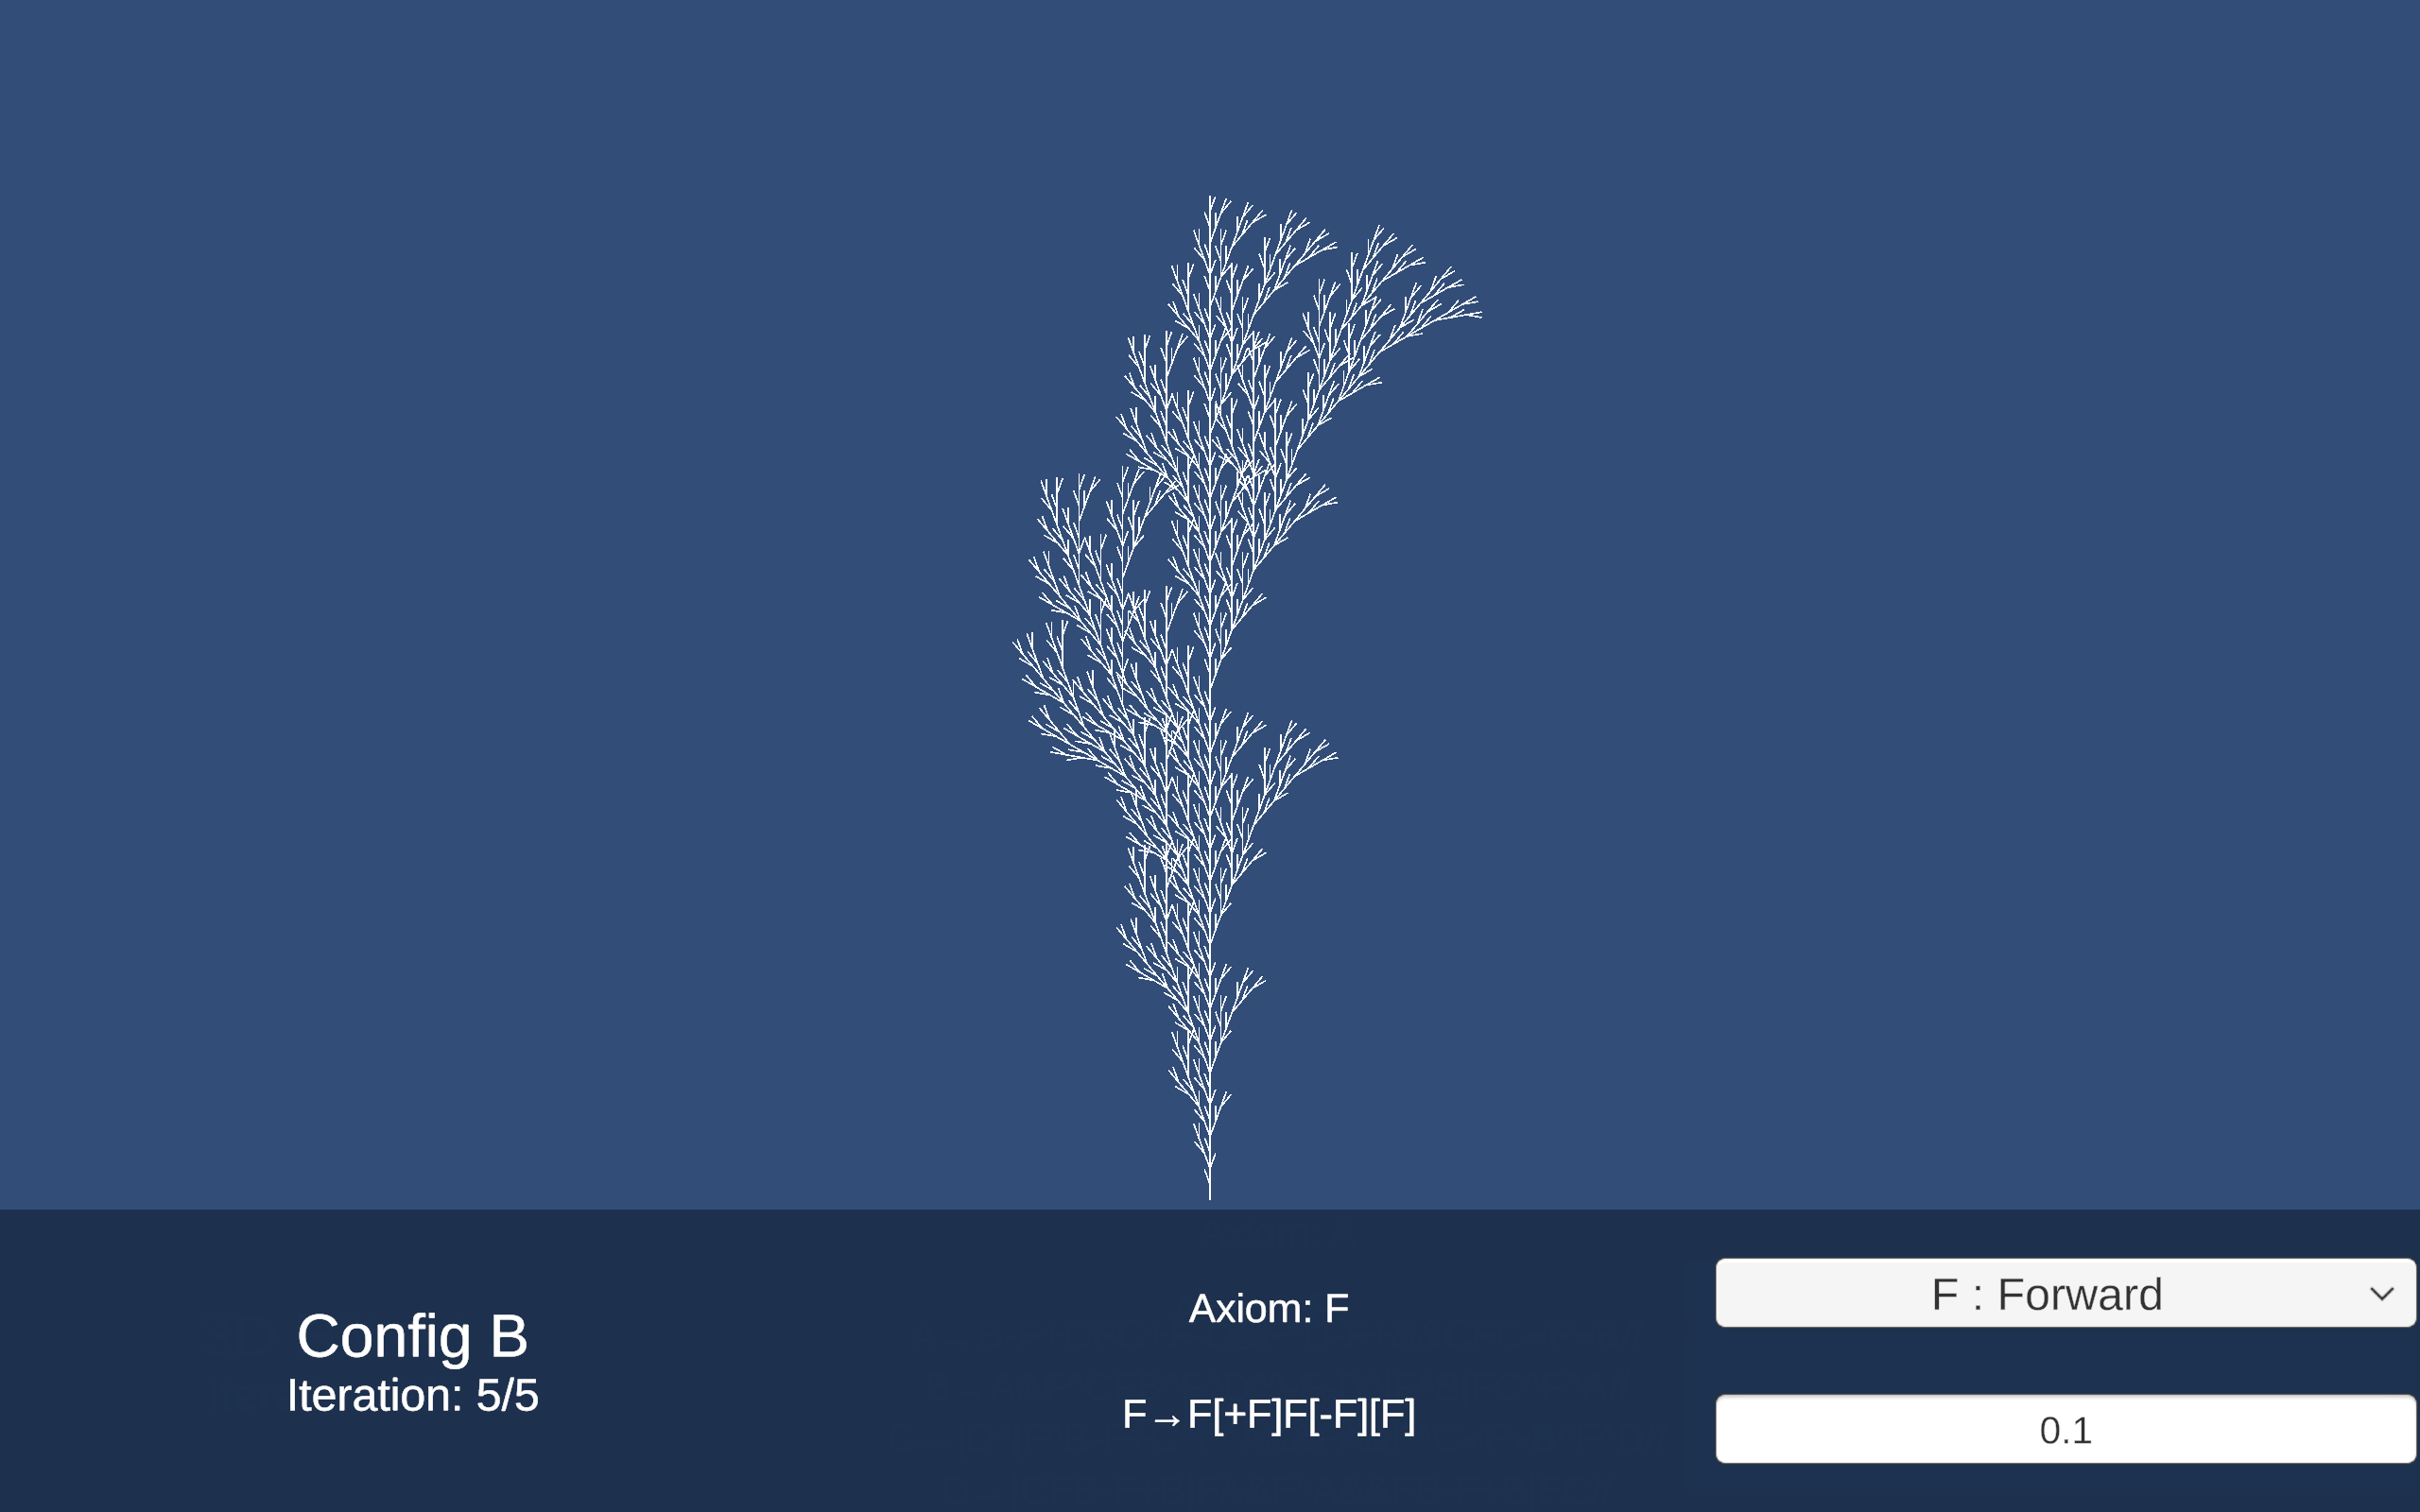
\includegraphics[width=.7\linewidth]{B.png}
\caption{$\delta$ = 20$^{\circ}$}
\end{subfigure}
\begin{subfigure}{1\textwidth}
\centering
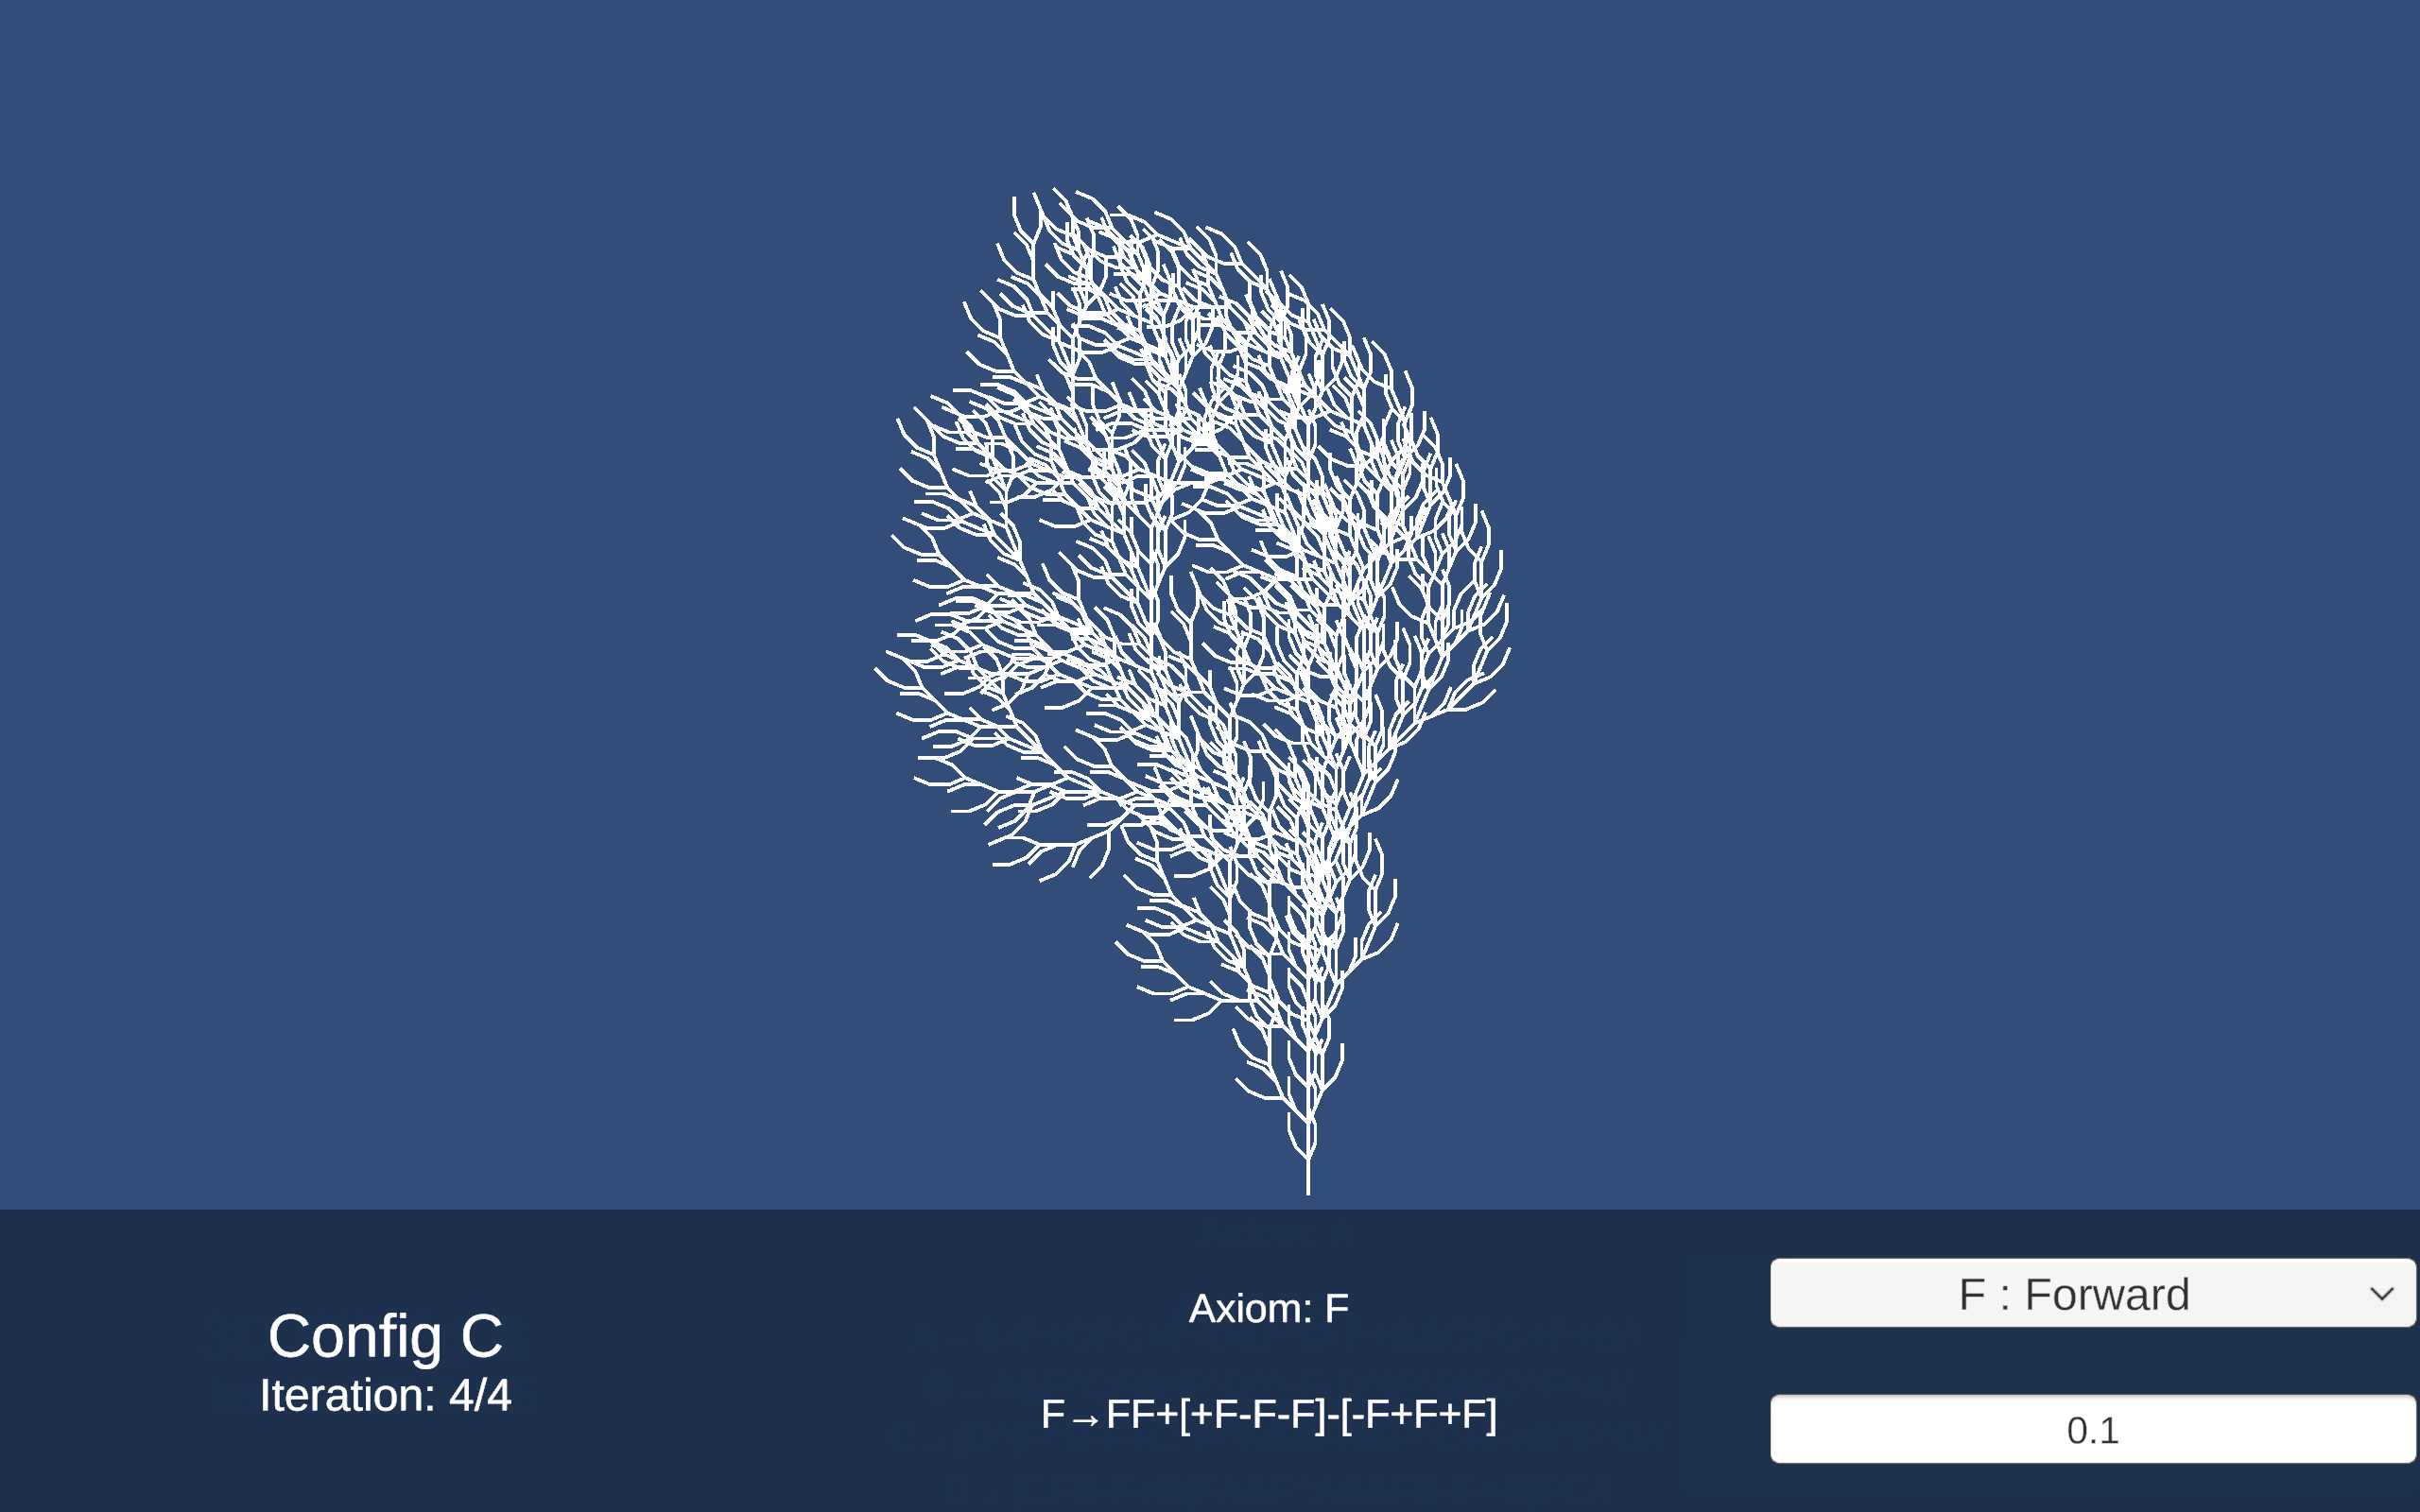
\includegraphics[width=.7\linewidth]{C.png}
\caption{$\delta$ = 22.5$^{\circ}$}
\end{subfigure}
\caption{Three 2D, Deterministic, Context-Free L-Systems Utilising Edge Replacement and Bracketing to Generate Branching Structures.}
\end{figure}

\begin{figure}
\begin{subfigure}{1\textwidth}
\centering
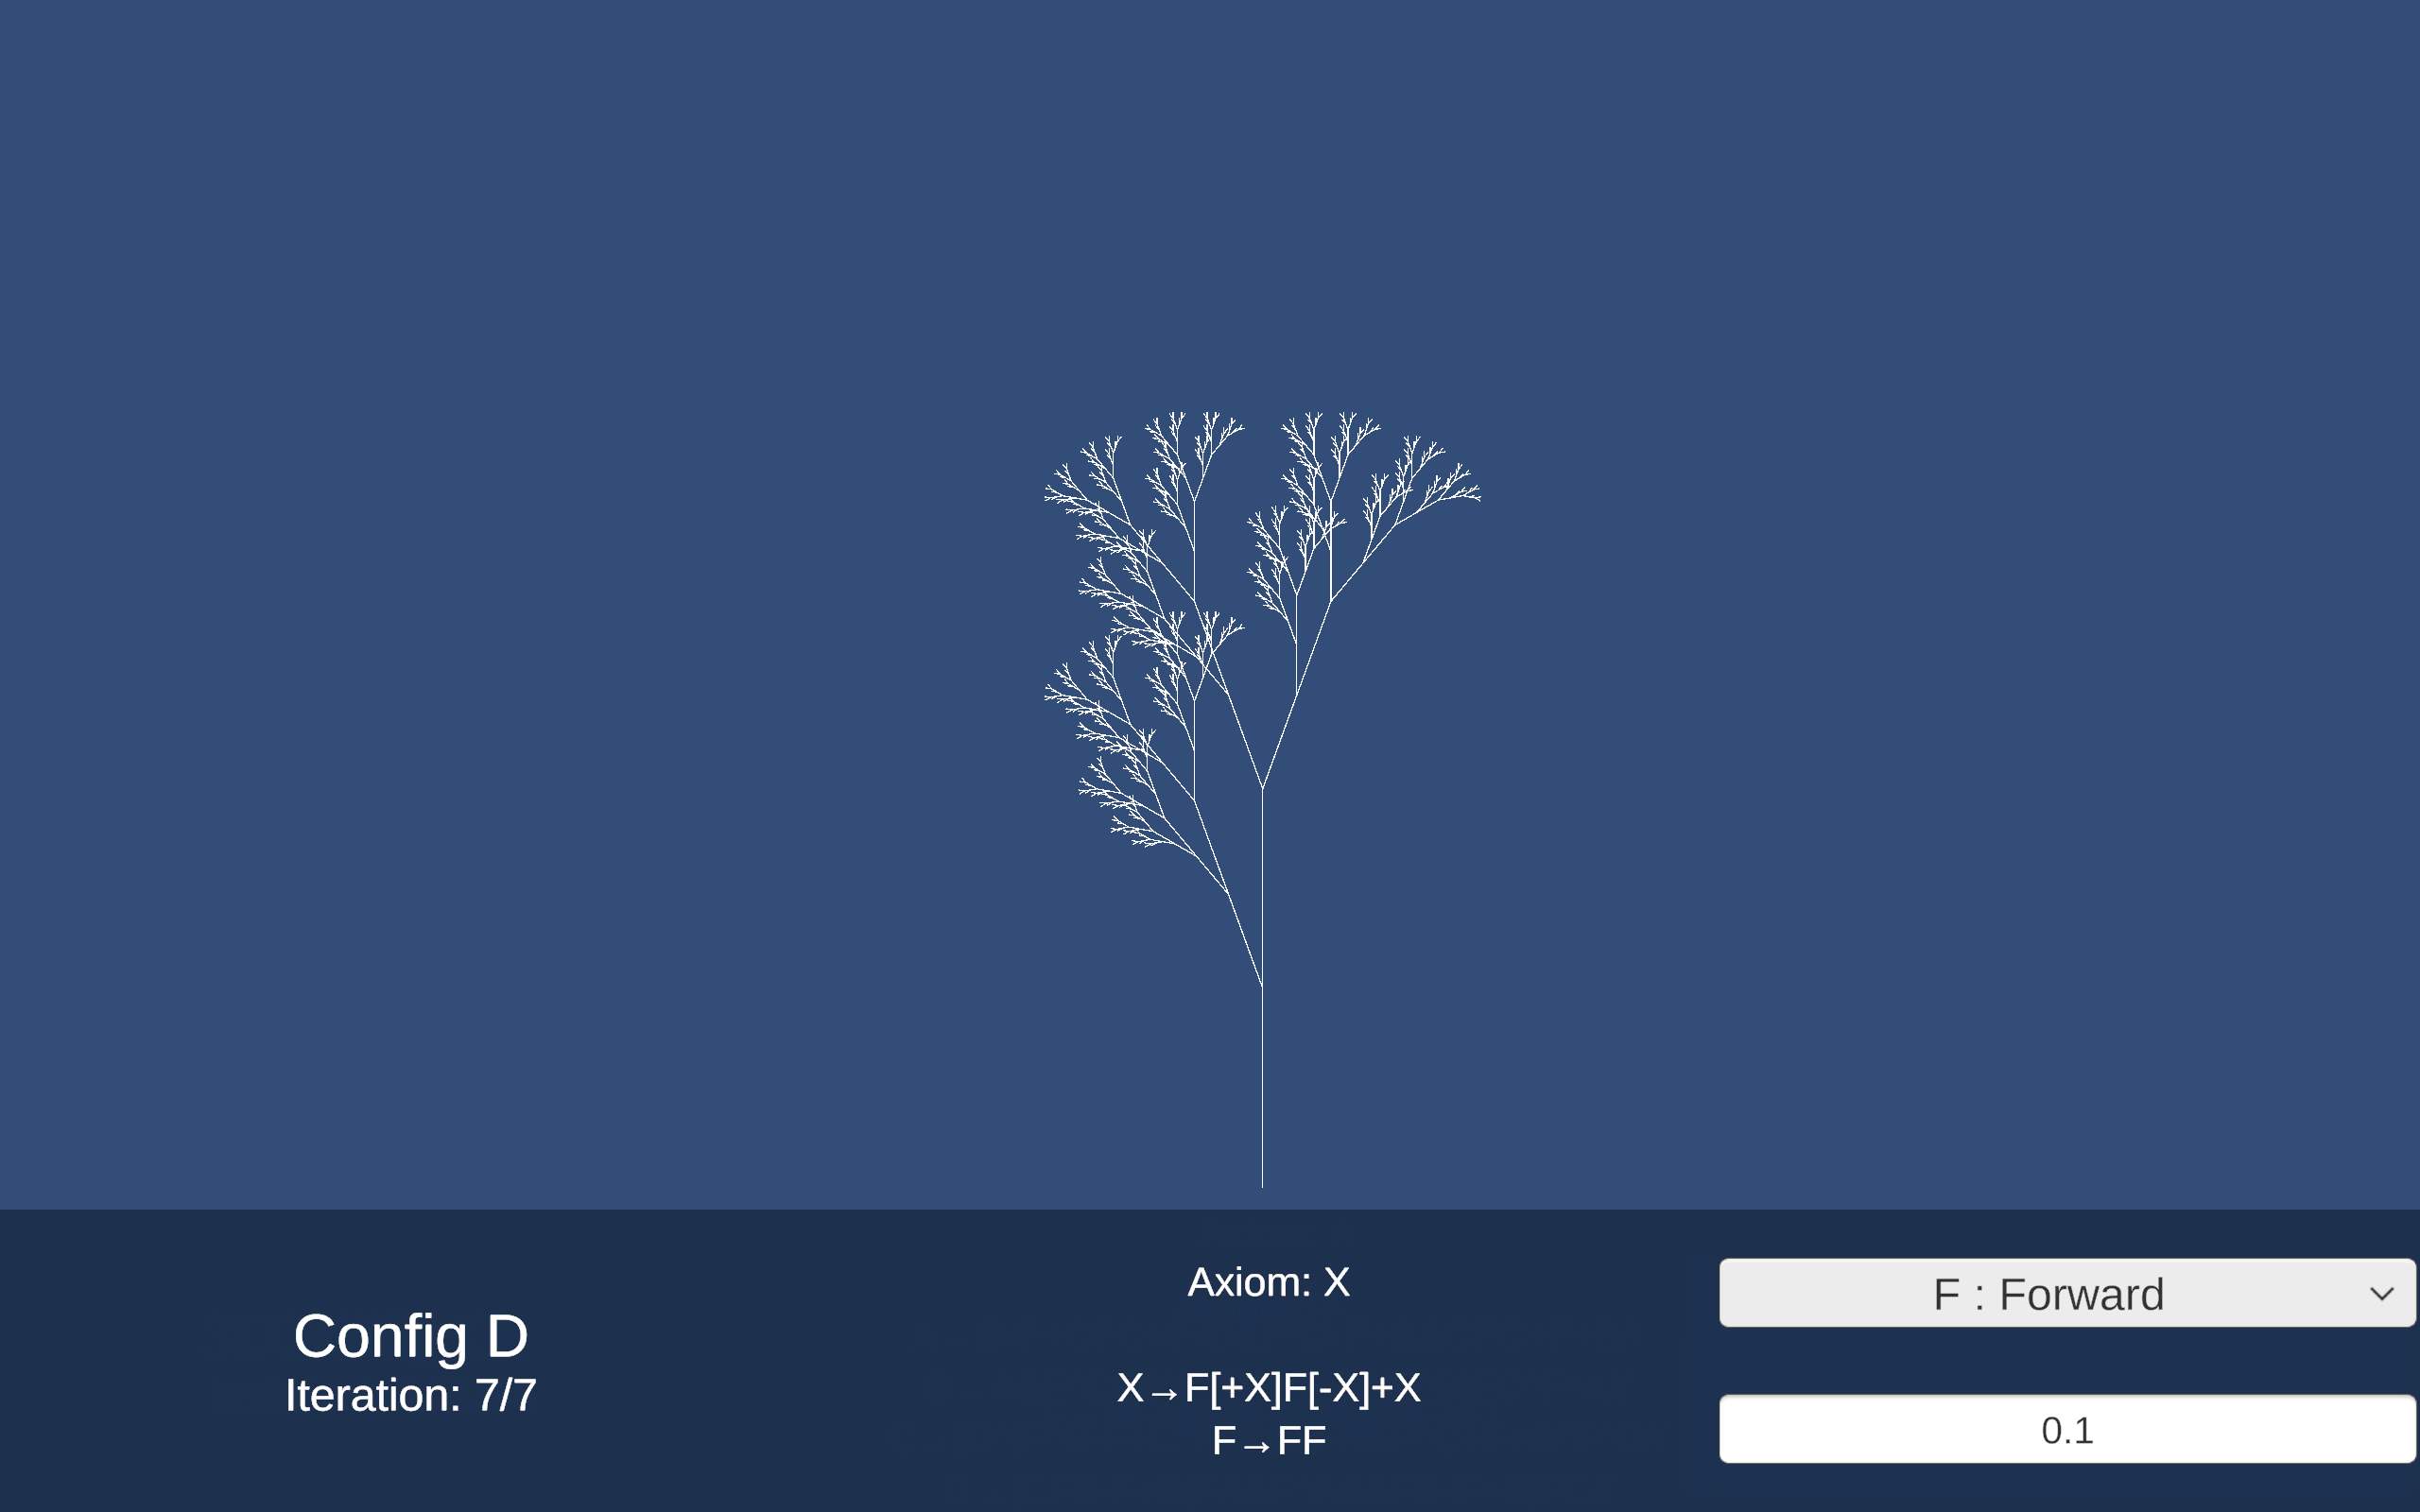
\includegraphics[width=.7\linewidth]{D.png}
\caption{$\delta$ = 20$^{\circ}$}
\end{subfigure}
\begin{subfigure}{1\textwidth}
\centering
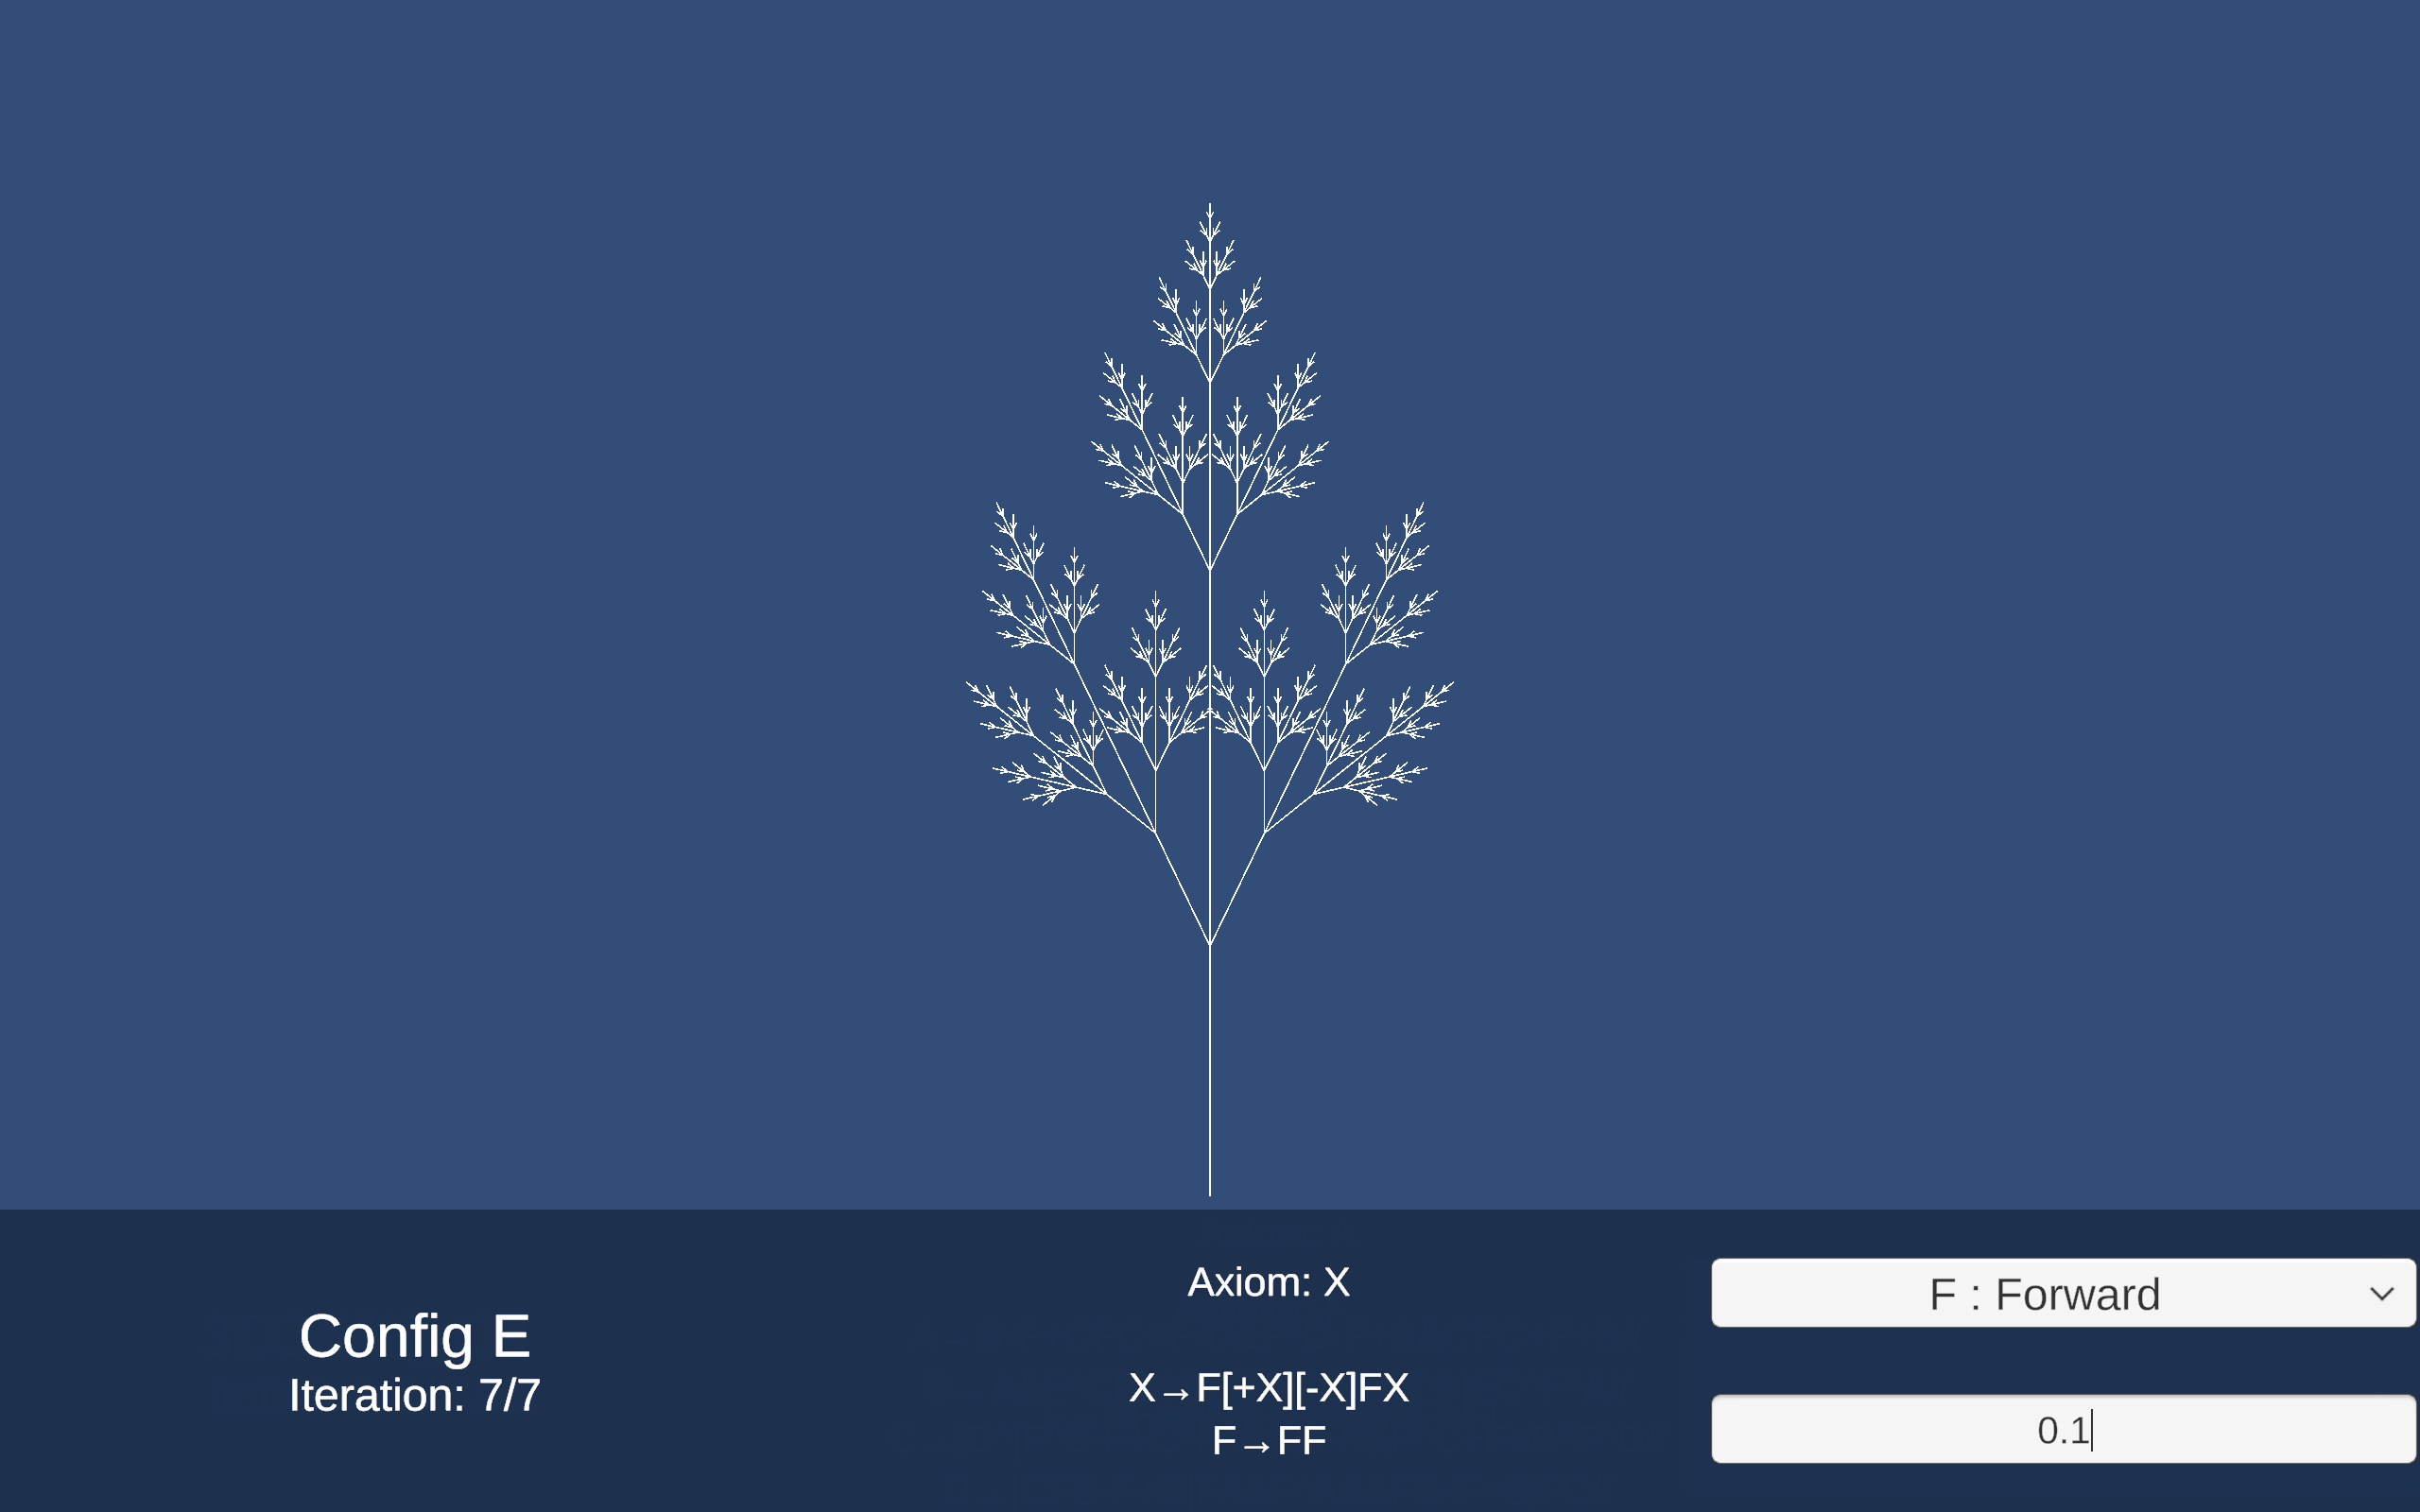
\includegraphics[width=.7\linewidth]{E.png}
\caption{$\delta$ = 25.7$^{\circ}$}
\end{subfigure}
\begin{subfigure}{1\textwidth}
\centering
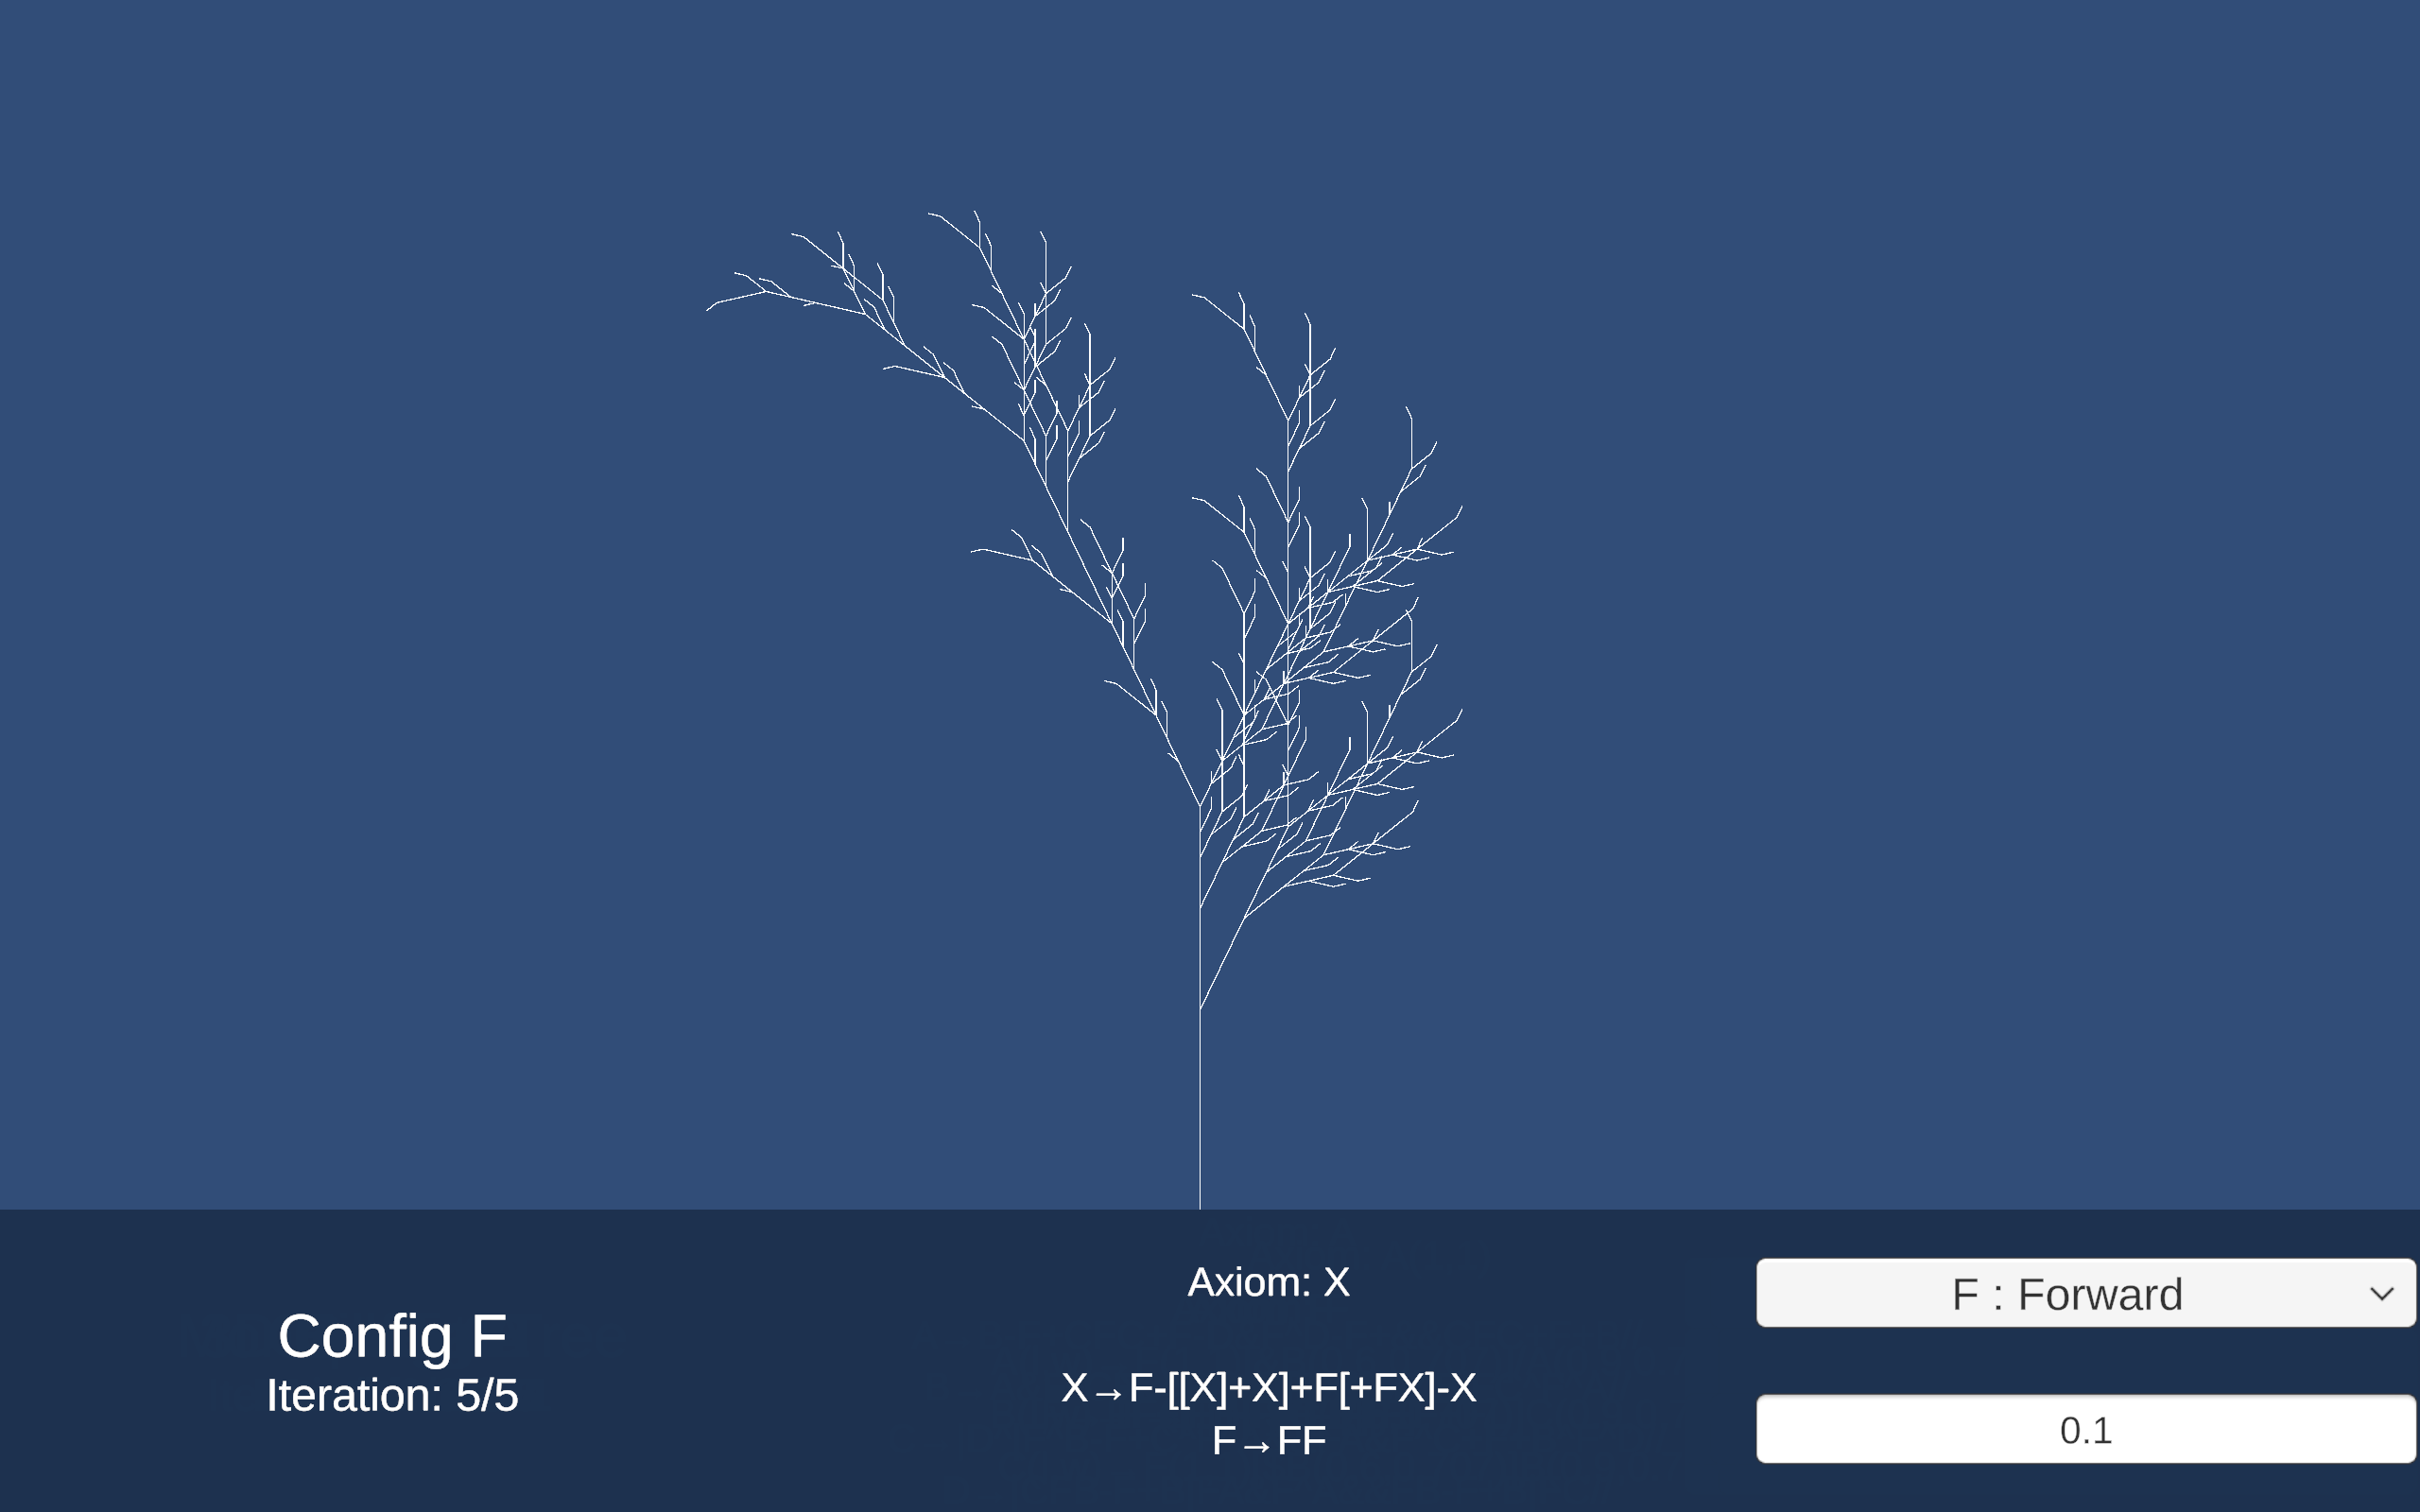
\includegraphics[width=.7\linewidth]{F.png}
\caption{$\delta$ = 22.5$^{\circ}$}
\end{subfigure}
\caption{Three 2D, Deterministic, Context-Free L-Systems Utilising Node Replacement and Bracketing to Generate Branching Structures.}
\end{figure}
\subsection{3D Hilbert Curve}
Figure 3 demonstrates the ability of this implementation to create complex 3D structures, with an extension of the Hilbert curve into 3D - as shown in \cite{abop}. This system implements 4 separate node-replacement rules, with all rotations set to 90$^{\circ}$. This structure is also not bracketed and consists of a single line - meaning it does not branch.
\begin{figure}
\centering
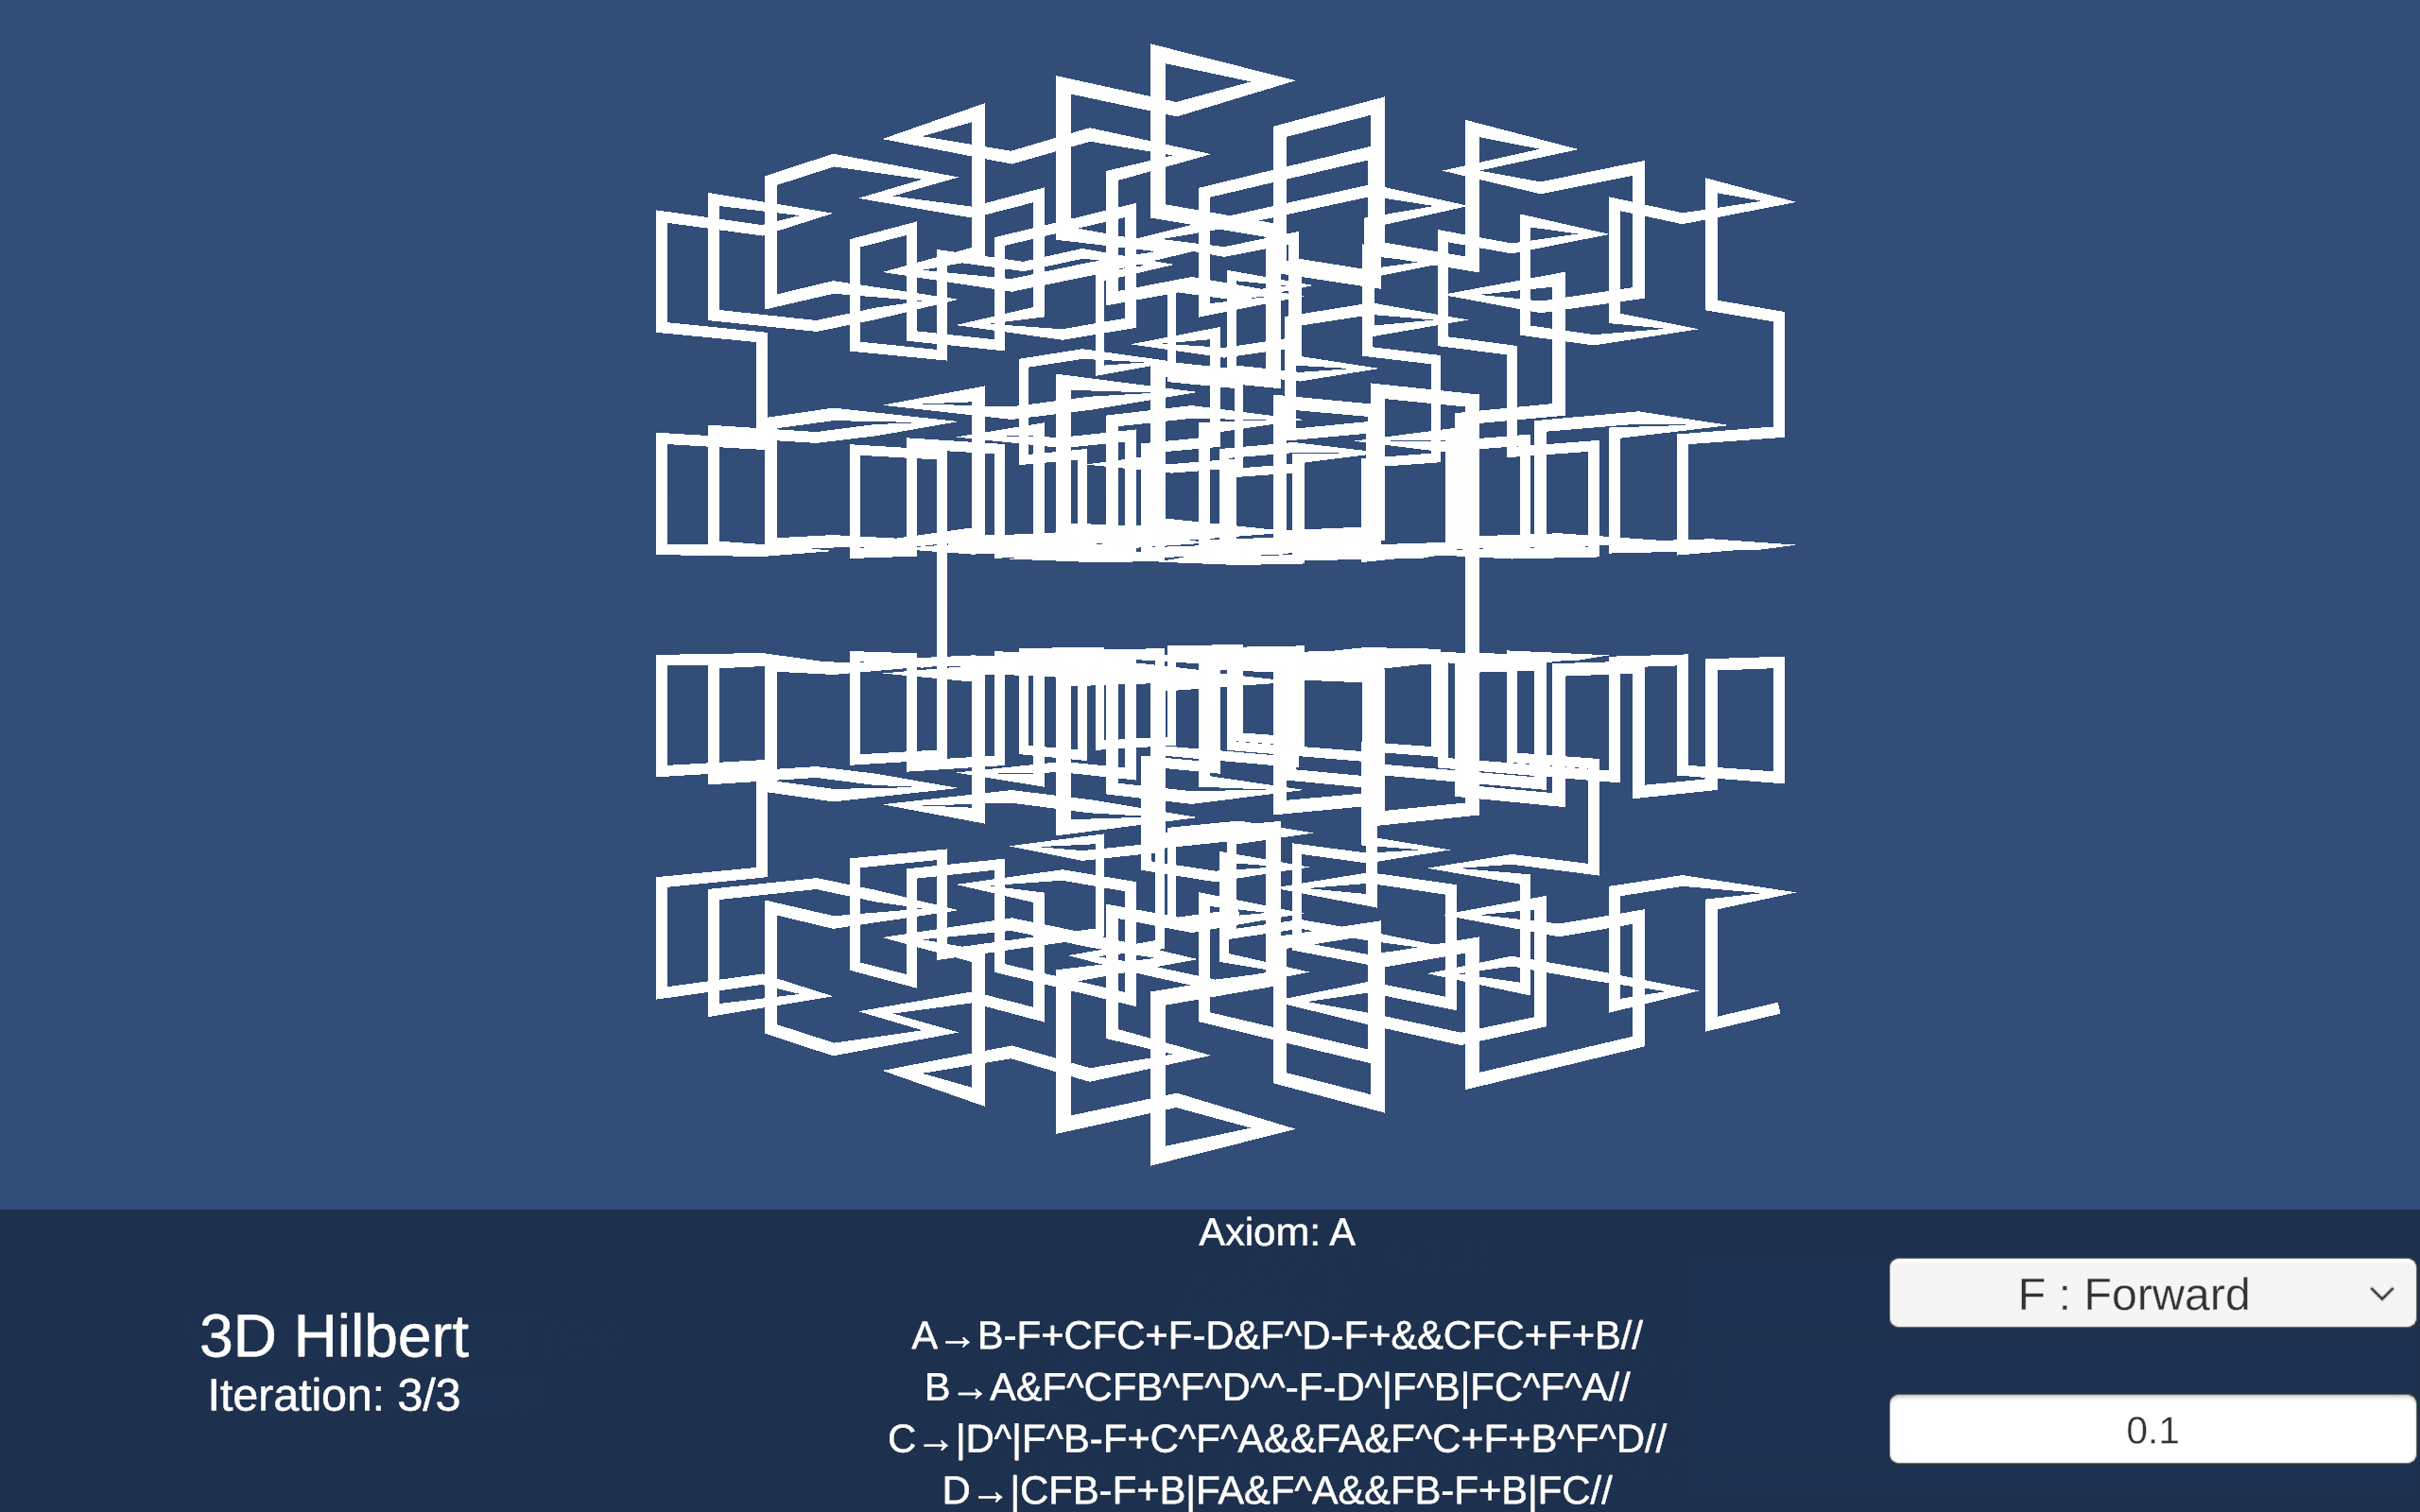
\includegraphics[width=1\linewidth]{Cube.png}
\caption{A 3D Extension of the Hilbert Curve, Inspired by \cite{abop}.}
\end{figure}

\subsection{Monopodial Tree}
Figure 4 shows a model of a monopodial tree, generated by a bracketed, parametric, 3D L-system - again inspired by work from \cite{abop}. The following angles are used for the model shown in figure 4:
\begin{center}
\begin{tabular}{c c}
-& -45$^{\circ}$\\\relax
\&& 45$^{\circ}$ \\\relax
/& 137.5$^{\circ}$\\
\end{tabular}
\end{center}
In this system  $-$ represents a branching angle from the lateral branches, $\&$ represents the branching angle from the trunk, and $/$ represents the angle around the trunk between different branches. This creates a \textit{monopodial} structure - where the main and lateral axes are clearly delineated.\\
There are two parameters used in this system - one for line length and one for line width. The trunk grows with a contraction ratio of 0.9 (meaning that new segments added to the trunk are 10\% each iteration), while the branches have a contraction ratio of 0.6. The width, meanwhile, has a decreasing rate of 0.707 each iteration - ensuring that a ``parent" branch has the same total diameter as two ``child" branches \cite{abop}. This creates the effect seen in figure 4, where the branches continuously get thinner as they get higher up the tree - something only possible due to the parametric aspect of the system.
\begin{figure}
\centering
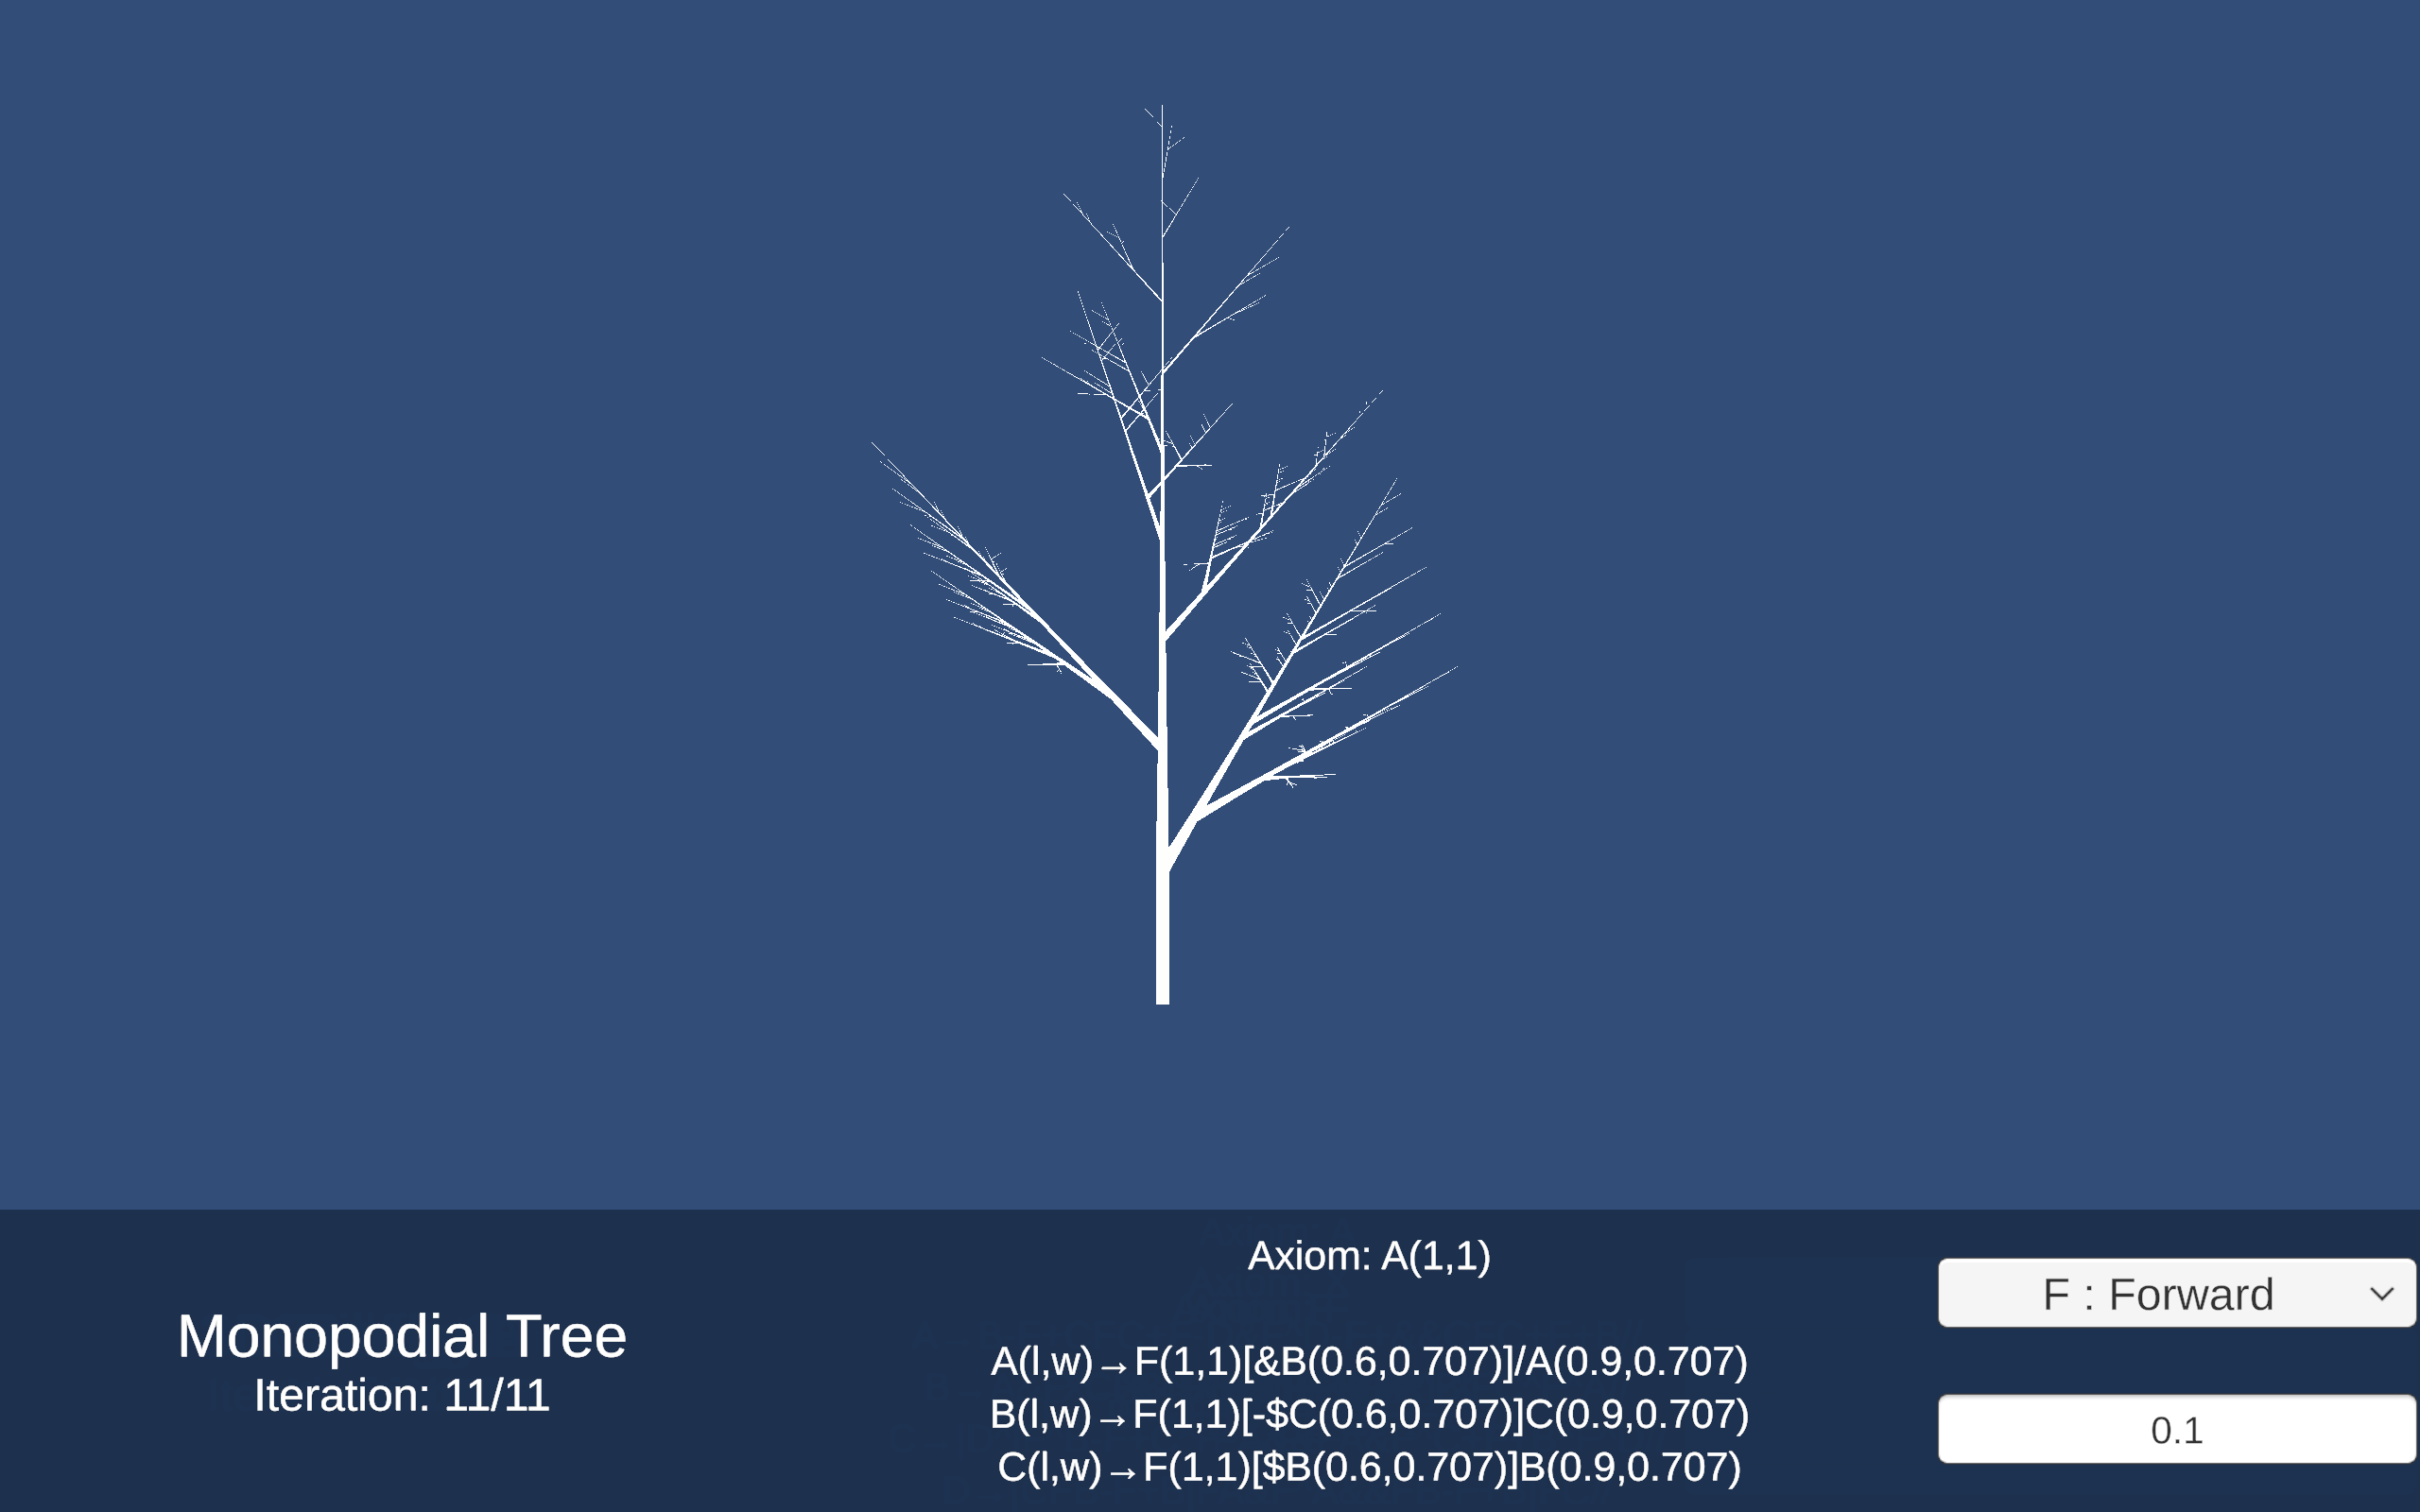
\includegraphics[width=1\linewidth]{TreeFig.png}
\caption{A Parametric L-System Used to Generate a Model of a Monopodial Tree.}
\end{figure}
\section{Conclusion}
The implemented system met all of the objectives detailed in section 2.5.1 - and is largely efficient, flexible, and robust. The monopodial tree in particular demonstrates the extent of the capabilities of the system, as it includes all of the techniques discussed within this report.\\
There are a few possible routes for expansion of this implementation, the first of which would be the design of a system to generate sympodial trees such as those found in \cite{abop} - which would be as simple as creating a new configuration file. Additionally, expanding the GUI to be able to modify the axiom, rules, and parameters would allow even greater control over the produced model. Next, there is the possibility of introducing further expansions upon the basic L-system - such as stochasticism or context-sensitivity. All the models created in this report were deterministic, but adding a random element to the model generation would allow the system to be more useful in 3D modelling contexts. Context-sensitivity also opens the door to the creation of more complex models and, as mentioned, some of the capability is already in place in the current system to allow that. Finally, the camera controls within the program could use some work. Currently, the camera position is automatically set based on the average value of all the points of the model. This largely works, but for some particularly top-heavy models it can cause some to be cut off. The ability to zoom the camera was added to reduce this, but adding a fully controllable camera would improve the experience.

\printbibliography
\end{document}